\pagestyle{empty} % Limpa o cabeçalho e o rodapé
\onehalfspacing % Espaçamento entre-linhas de 1,5
% \hyphenpenalty=10000 % To prevent hyphenation
\pretolerance=10000 % To avoif overful lines
%\selectlanguage{english}
\selectlanguage{brazilian}
\pagenumbering{arabic} % Números das páginas em arábicos
\newcounter{ex} % counter for exercises
\renewcommand{\chaptername}{Tutorial}
\chapter{Introdução ao Linux}\label{tut1}
\rhead{\tiny Instituto de Biociências --USP: BIZ0433 - Inferência Filogenética: Filosofia, Método e Aplicações}
\cfoot{\tiny \cc \ccby \ccsa \href{http://creativecommons.org/licenses/by-sa/4.0/}{Creative Commons Attribution-ShareAlike 4.0 International License}}
%\vspace{5pt}
{\large \sc BIZ0433 - Inferência Filogenética: Filosofia, Método e Aplicações.}\par
%\vspace{10pt}
\par
\minitoc % for table of contents within the chapter
\newpage
\section*{}\addcontentsline{toc}{section}{Objetivo}
\onehalfspacing
\vspace*{5pt}
\begin{center}
\emph{\begin{large}Objetivo\end{large}}\label{tut1:Objetivo}
\vspace{2pt}
\end{center}
%% TEXTO DO RESUMO
Este tutorial foi, em grande parte, copiado de uma apostila que encontrei nos servidores do IME/USP cujo objetivo era introduzir os sistema Lunix para principiantes. Como não constava nenhuma informação sobre os autores do documento, não pude dar devido crédito ao que foi inserido aqui.\\

O Objetivo deste tutorial é fazer com que o aluno entenda os princípios básicos do sistema operacional Linux, principalmente no que concerne ao uso de terminais (\textit{i.e.}, modo texto) e comandos de linha na execução de tarefas básicas tais como, movimentação dentro do sistema operacional, criação de diretórios e arquivos, entre outros. Esse tutorial é fundamental para aqueles que estão matriculados nesse curso, uma vez que toda disciplina será baseada neste sistema operacional. No entanto, o aluno não deve ter a expectativa de que todos os comandos apresentados aqui serão absorvidos no primeiro contato. A proficiência nesses comandos vem com o tempo, e é um aprendizado que requer constante aprimoramento, pois sempre se aprende algo de novo. Portanto, este tutorial deverá ser sempre usado como referência para as demais aulas.\\
%\pagenumbering{arabic} % Números das páginas em arábicos --> moved to line 8
\newpage
\pagestyle{fancy} % Inclui o cabeçalho definido no meta.tex
\begin{refsection}
\renewcommand*{\finalnamedelim}{\addspace\&\space}% Usar '&' ao invés de 'e'.

%% O QUE É LINUX (copiada da apostila do IMA - atribuir autoria)
\section{O que é Linux?}\label{tut1:linux}
O termo Linux é usado em vários contextos com significados diferentes. A rigor, Linux é um kernel. No entanto, em alguns contextos, Linux significa sistema operacional (não qualquer sistema operacional, mas um que use o kernel Linux).\\

\textbf{Sistema Operacional:} é um \textit{software} que serve de interface entre o computador e o usuário, gerenciando recursos (como memória, processamento, entre outros).\\

\textbf{Kernel:} é o núcleo ou cerne do sistema operacional (é a parte deste que fica mais ``próxima'' do hardware).\\

Você pode agora estar se perguntando se deve chamar apenas o kernel de Linux. Como dito anteriormente, a rigor, Linux é o kernel. Contudo, a expressão ``sistema operacional Linux'' tornou-se muito difundida. Outra pergunta pode ter surgido neste ponto: qual o nome do sistema operacional então? Mais uma controvérsia aqui. Quando algum usuário instala ''o Linux'', ele está instalando o kernel e mais uma série de outros \textit{softwares} (\textit{i.e.}, aplicativos ou programas). Grande parte desses aplicativos pertence a um projeto chamado GNU. Logo, o sistema operacional formado pelo kernel mais utilitários e aplicativos, como defendem alguns, deveria ser chamado de GNU/Linux.\\

\subsection{Um breve histórico - Como surgiram o GNU e o Linux:}\label{tut1:linux:history}
No ano de 1984, Richard Stallman iniciou o Projeto GNU, que tinha por objetivo criar um sistema operacional que fosse totalmente livre. Esse sistema operacional deveria ser compatível com outro sistema operacional - o UNIX (daí o nome GNU - GNU is Not Unix). No ano seguinte, Stallman fundou a FSF (\textit{Free Software Foundation}), com o propósito de eliminar restrições de uso, cópia e distribuição de \textit{software}.\\
Por volta de 1991, o sistema GNU estava quase pronto, exceto pelo kernel. Stallman estava trabalhando no desenvolvimento de um kernel chamado Hurd. Ao mesmo tempo, o finlandês Linus Torvalds havia criado um kernel compatível com as aplicações do projeto GNU. A esse kernel foi dado o nome de Linux. Atualmente, Linux tornou-se um termo genérico para se referir a sistemas operacionais ''Unix-like'' baseados no kernel Linux. Tornou-se, também, o melhor exemplo de Software Livre e de código aberto.\\

\subsection{Software Livre e Licença GPL:}\label{tut1:linux:gpl}
Na Seção anterior, foi dito que Stallman pretendia criar um sistema operacional livre e que o GNU/Linux era um exemplo de Software Livre. A definição de Software Livre, dada pela FSF é:\\
\begin {myindentpar}{0.5cm}
\begin{enumerate}[\itshape i.]
 \item{Executar o \textit{software} com qualquer propósito (liberdade nº 0).}
 \item{Estudar o funcionamento do \textit{software} e adaptá-lo às suas necessidades (liberdade nº 1).}
 \item{Redistribuir (inclusive vender) cópias do \textit{software} (liberdade nº 2).}
 \item{Melhorar o programa e tornar as modificações públicas para que a comunidade inteira se beneficie da melhoria (liberdade nº 3).}
\end{enumerate}
\end{myindentpar}

	Ao contrário do que as pessoas pensam, Software Livre (do inglês \textit{Free Software}) não é sinônimo de gratuito. O que ocorre é uma confusão envolvendo a palavra ''\textit{free}'' em inglês, que significa tanto gratuito como livre. Mas o sentido que Stallman queria dar era de ``livre''. De qualquer forma, a maioria dos \textit{softwares} livres é distribuída de forma gratuita. Grande parte dos projetos de \textit{software} livre (incluindo o GNU/Linux) é distribuída sob a GPL (\textit{General Public License} - Licença Pública Geral), que é a licença idealizada por Stallman e que se baseia nas quatro liberdades citadas anteriormente. Com a garantia destas liberdades, a GPL permite que os programas sejam distribuídos e reaproveitados, mantendo, porém, os direitos do autor de forma a não permitir que essa informação seja usada de uma maneira que limite as liberdades originais. 

\subsection{Distribuições:}\label{tut1:linux:dist}
Distribuições Linux (também chamadas Distribuições GNU/Linux ou simplesmente distros) consistem em ``pacotes'' de \textit{software} baseados no kernel Linux que incluem determinados tipos de \textit{software} para satisfazer as necessidades de um grupo específico de usuários, dando assim origem a versões domésticas, empresariais e para servidores.\\
Exemplos de Distribuições Linux: Ubuntu, Debian, Slackware, Fedora, Red Hat, Arch, Gentoo, Mandriva, openSUSE etc.\\
Qual é a melhor distribuição é uma questão de necessidade e gosto. Apresentamos a seguir uma breve descrição de algumas distros, para que você possa ter uma ideia de suas principais características.\\
\begin {myindentpar}{0.5cm}
\begin{enumerate}[\itshape i.]
 \item \textit{Debian:}\label{tut1:linux:dist:debian}\\
	A distro Debian (ou Debian GNU/Linux) é desenvolvida pelo \href{http://www.debian.org/distrib/}{Projeto Debian}, um grupo de voluntários mantido por doações através da organização sem fins lucrativos Software in the Public Interest (SPI).\\
	Debian baseia-se fortemente no projeto GNU e tem como principais características um alto compromisso com estabilidade e segurança bem como uma grande facilidade no que concerne à instalação de programas, através de um gerenciador de pacotes completo (dpkg) e sua interface (apt), utilizados amplamente em outras distribuições.\\
	A última versão estável desta distro é 7.8 de 10 de janeiro de 2015.\\
 \item \textit{Red Hat Entreprise Linux:}\label{tut1:linux:dist:redhat}\\
	Red Hat Enterprise Linux é uma distro criada pela empresa norte-americana \href{https://br.redhat.com/products/enterprise-linux/}{Red Hat}. O foco desta distribuição é o mercado corporativo, incluindo versões para servidores e para desktops.\\
	O Red Hat Enterprise Linux não possui um ciclo de lançamentos fixo: a versão atual é a 7 de 2015.\\
 \item \textit{Slackware:}\label{tut1:linux:dist:slackware}\\
	Simplicidade e estabilidade são duas características marcantes na distribuição do \href{http://www.slackware.com}{Slackware}. Muito comum em servidores, procura ser uma distribuição ``leve'', praticamente sem enfeites e rápida, muito apreciada por usuários mais experientes.\\
	Encontra-se atualmente na versão Slackware 14.1.\\
 \item \textit{Ubuntu:}\label{tut1:linux:dist:ubuntu}\\
	Ubuntu é uma distro GNU/Linux baseada na distro Debian e é patrocinada pela \href{http://www.ubuntu.com/}{Canonical}. A proposta do Ubuntu é oferecer um sistema operacional que qualquer pessoa possa utilizar sem dificuldades, independentemente de nacionalidade, nível de conhecimento ou limitações físicas (a palavra Ubuntu é de origem africana e significa ``humanidade para os outros''). Essa distro oferece um ambiente atualizado e estável, focado na usabilidade e na facilidade de sua instalação.\\
	A cada seis meses, uma nova versão da distro é lançada, a versão atual com suporte longo prazo é Ubuntu 14.04.2 LTS (Trusty Tahr). Os números 14 e 4 são, respectivamente, o ano e o mês do lançamento da versão e a sigla LTS significa ``\textit{long time support}'' que é geralmente de 5 anos. \\
\end{enumerate}
\end{myindentpar}

\subsection{Aplicativos, diretórios e arquivos:}\label{tut1:linux:struct}

\begin {myindentpar}{0.5cm}
\begin{enumerate}[\itshape i.]
 \item \textit{Aplicativos:}\\
Basicamente, para qualquer programa que você utilizava no Windows, existe uma alternativa no GNU/Linux. Por outro lado, vários dos aplicativos inicialmente concebidos sob ``GNU/Linux'' também estão disponíveis na versão para Windows (\textit{e.g.}, VLC). Caso você queira saber quais programas são equivalentes entre Linux e Windows, consulte \href{http://wiki.linuxquestions.org/wiki/Linux_software_equivalent_to_Windows_software}{esta página}.
%
  \item \textit{Visão geral da organização dos arquivos no Linux:}\\
	Grosso modo, pode-se dizer que, no Linux, tudo é arquivo. Se há algo que não seja um arquivo, então este algo é um processo. No GNU/Linux (como no UNIX), não há diferença entre arquivo e diretório, uma vez que um diretório é apenas um arquivo contendo nomes de outros arquivos. Imagens, músicas, textos, programas, serviços e assim por diante são todos arquivos. Dispositivos de entrada e saída, e geralmente, todos os dispositivos, são considerados como arquivos. Todos estes arquivos estão organizados de acordo com uma hierarquia, isto é, há critérios que prevêm os principais diretórios e seu conteúdo (veja Figura \ref{tut1:fig:fs}). Estes critérios são definidos por um padrão, o FHS (\textit{Filesystem Hierarchy Standard}).\\
%%%%%%%%%%%%%%%%%%%%%%%%%%% FIGURA DO FILE SYSTEM %%%%%%%%%%%%%%%%%%%%%%%%%%%
%  \vspace{-1em}
  \begin{figure}[H]
    %\ffigbox[\FBwidth]
      {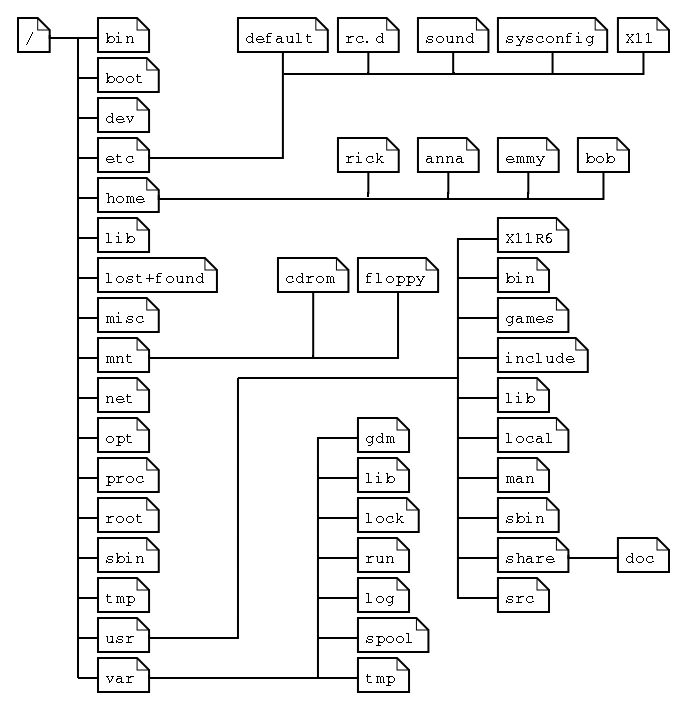
\includegraphics[scale=1]{figures/tut1/fs_layout.eps}}
      {\caption[\textit{Lunux File System}]{Estrutura hierárquica do \textit{file system} do Linux.}\label{tut1:fig:fs}}
  \end{figure}
%%%%%%%%%%%%%%%%%%%%%%%%%%% FIM DA FIGURA DO FILE SYSTEM %%%%%%%%%%%%%%%%%%%%%%%%%%%
No topo da hierarquia de arquivos fica o chamado diretório raiz (ou, mais apropriadamente, diretório \textit{root}), pois a estrutura de diretórios é chamada também de ``Árvore de Diretórios''. Vejamos alguns exemplos citando os principais diretórios do sistema:\\

  \subitem {\textbf{/}}: Chamado diretório root, é o diretório principal do sistema. Dentro dele estão todos os diretórios do sistema.
  \subitem {\textbf{/bin}}: Contém comandos e programas essenciais para todos os usuários (alguns desses comandos serão tratados adiante).
  \subitem {\textbf{/boot}}: Contém arquivos necessários para a inicialização do sistema.
  \subitem {\textbf{/dev}}: Contém referências para todos os dispositivos, os quais são representados como arquivos com propriedades especiais.
  \subitem {\textbf{/etc}}: Contém arquivos de configuração.
  \subitem {\textbf{/home}}: Contém os diretórios dos usuários.
  \subitem {\textbf{/lib}}: Contém bibliotecas (que são subprogramas ou códigos auxiliares utilizados por programas) essenciais para o funcionamento do Linux, e também os módulos do kernel.
  \subitem {\textbf{/media}}: Contém subdiretórios que são usados como pontos de montagem para mídias removíveis, cdroms, discos externos e pen drives, entre outros.
  \subitem {\textbf{/root}}: Este é o diretório ``home'' do super usuário (usuário root). Não confundir com o diretório root, o /. O diretório /root contém os arquivos do usuário root. O diretório / é o topo da hierarquia de arquivos. \textbf{Usuário root} é o administrador do sistema, possui acesso a todos os comandos e arquivos.
  \subitem {\textbf{/tmp}}: Contém arquivos temporários.
  \subitem {\textbf{/usr}}: Contém programas, bibliotecas, entre outros arquivos.
    \subsubitem {\textbf{/usr/bin}}: Contém os binários de programas não-essenciais (os essenciais ficam no /bin).
    \subsubitem {\textbf{/usr/src}}: Contém os códigos-fonte de alguns programas instalados no sistema.
  \subitem {\textbf{/var}}: Contém arquivos ``variáveis'', como logs, base de dados.
    \subsubitem {\textbf{/var/log}}: Como o próprio nome diz, possui arquivos de log. \textbf{Arquivo de log:} é um arquivo que armazena registros de eventos relevantes de um programa ou do sistema.
    \subsubitem {\textbf{/var/run}}: Contém informações sobre a execução do sistema desde a sua última inicialização.

  \item \textit{Caminho absoluto vs. Caminho relativo:}\\
Caminho de um diretório (ou de um arquivo) é composto pelos diretórios que devemos percorrer até chegar a ele. Vamos diferenciar caminho absoluto de caminho relativo por meio de um exemplo.\\
Consideremos, por exemplo, o diretório xinit/. Consideremos que este diretório encontra-se dentro de um outro diretório, o diretório X11/. Este X11/, por sua vez, está dentro do diretório etc/, que, finalmente, está sob o diretório root, o /.\\
O raciocínio inverso seria: temos o / e dentro o etc/ (/etc/), e dentro o X11/ (/etc/X11) que contém o xinit/ (/etc/X11/xinit). Logo, ``/etc/X11/xinit/'' é o \textbf{caminho absoluto} (``\textit{absolut path}'') para o diretório xinit, ou seja, são os diretórios que devemos percorrer, começando pelo /, até o diretório xinit/.\\
Consideremos agora os mesmos diretórios do caso anterior (/etc/X11/xinit/). Suponhamos agora que estamos no diretório etc/. Para dizer qual é o caminho do diretório xinit/, bastaria dizer apenas X11/xinit - este é o \textbf{caminho relativo} (``\textit{relative path}'') do diretório (em relação ao diretório /etc -- é seu \textbf{diretório de trabalho}). Se estivéssemos no diretório X11/, o \textbf{caminho relativo} seria simplesmente xinit/.\\
Em suma, caminho absoluto é aquele que utiliza toda a estrutura de diretórios, ao passo que o relativo toma um diretório como referência e define o caminho a partir daí.\\

  \item \textit{Permissões de acesso:}\\
O Linux foi desenvolvido para ser um sistema multi-usuário. Isto significa que vários usuários podem ter configurações personalizadas, independentes das configurações dos demais usuários, bem como diferentes usuários podem executar tarefas ao mesmo tempo numa mesma máquina. Assim sendo, cada usuário pode querer negar ou permitir o acesso a determinado arquivo ou diretório. Por isso, existem as chamadas permissões de acesso do Linux: para impedir o acesso indevido de outros usuários ou mesmo de programas mal intencionados a arquivos e diretórios.\\
Mostraremos algumas destas permissões nesta seção. Mais adiante, mostraremos como manipulá-las.

 \item \textit{Donos, grupos e outros:}\\
  No Linux, para cada arquivo são definidas permissões para três tipos de usuários: o \textbf{dono} do arquivo, um \textbf{grupo} de usuários e os demais usuários (\textbf{outros}, que não são nem o dono, nem pertencem ao grupo).\\
	\subsubitem{\textbf{Dono}}: é o usuário que criou o mesmo, seu dono. Somente o dono e o usuário root podem mudar as permissões para um arquivo ou diretório.
	\subsubitem{\textbf{Grupo}}: é um conjunto de usuários. Grupos foram criados para permitir que vários usuários tivessem acesso a um mesmo arquivo.
	\subsubitem{\textbf{Outros}}: são os usuários que não se encaixam nos tipos de usuários supracitados.

 \item \textit{Tipos de permissões:}\\
 Os três tipos básicos de permissão para arquivos e diretórios são:\\
	\subsubitem{\textbf{r} (read):} permissão de leitura para arquivos. Caso seja um diretório, permite listar seu conteúdo (com o comando ls, por exemplo - que será visto adiante).
	\subsubitem{\textbf{w} (write):} permissão de escrita para arquivos. Caso seja um diretório, permite a gravação de arquivos ou outros diretórios dentro dele. Para que um arquivo/diretório possa ser apagado, é necessário o acesso à escrita (gravação).
	\subsubitem{\textbf{x} (execute):} permite executar um arquivo. Caso seja um diretório, permite que seja acessado através do comando cd (você verá este comando também adiante, equivale a ''entrar'' no diretório).

 Em suma, para cada arquivo do sistema, são definidas permissões para o dono do arquivo, para um grupo de usuários e para os demais usuários. Essas permissões são de leitura, escrita e execução (r, w ou x). Você entenderá melhor estes conceitos adiante, mas tente familiarizar-se com eles desde já.\\

\end{enumerate}
\end{myindentpar}

\section{Modo texto}\label{tut1:text_mode}
 Não é apenas pelo modo gráfico que o usuário consegue interagir com o sistema. É possível fazer isso pelo modo texto, digitando comandos e nomes de programas para conseguir uma ``resposta'' do sistema. Por isso, o modo texto é também chamado de linha de comando.\\
É importante para um usuário do GNU/Linux aprender a trabalhar no modo texto por vários motivos: otimiza várias tarefas, existem alguns programas que só podem ser executados no modo texto e também porque o modo gráfico consome mais recursos computacionais.\\
Há duas formas de acessar o modo texto do sistema. Você pode acessar um terminal ``puro'', pressionando as teclas ``Ctrl+Alt+F1'' simultanemamente. Na verdade, você pode substituir a tecla F1 por F2, F3, etc até F6. Isso lhe permite iniciar seis seções simultâneas no modo texto. Para retornar ao modo gráfico, basta pressionar as teclas ``Ctrl+Alt+F7''! Veja como o modo texto se parece na Figura \ref{tut1:fig:terminal0}).\\

%%%%%%%%%%%%%%%%%%%%%%%%%%% FIGURA DO TERMINAL %%%%%%%%%%%%%%%%%%%%%%%%%%%
%  \vspace{-1em}
  \begin{figure}[H]
    %\ffigbox[\FBwidth]
      {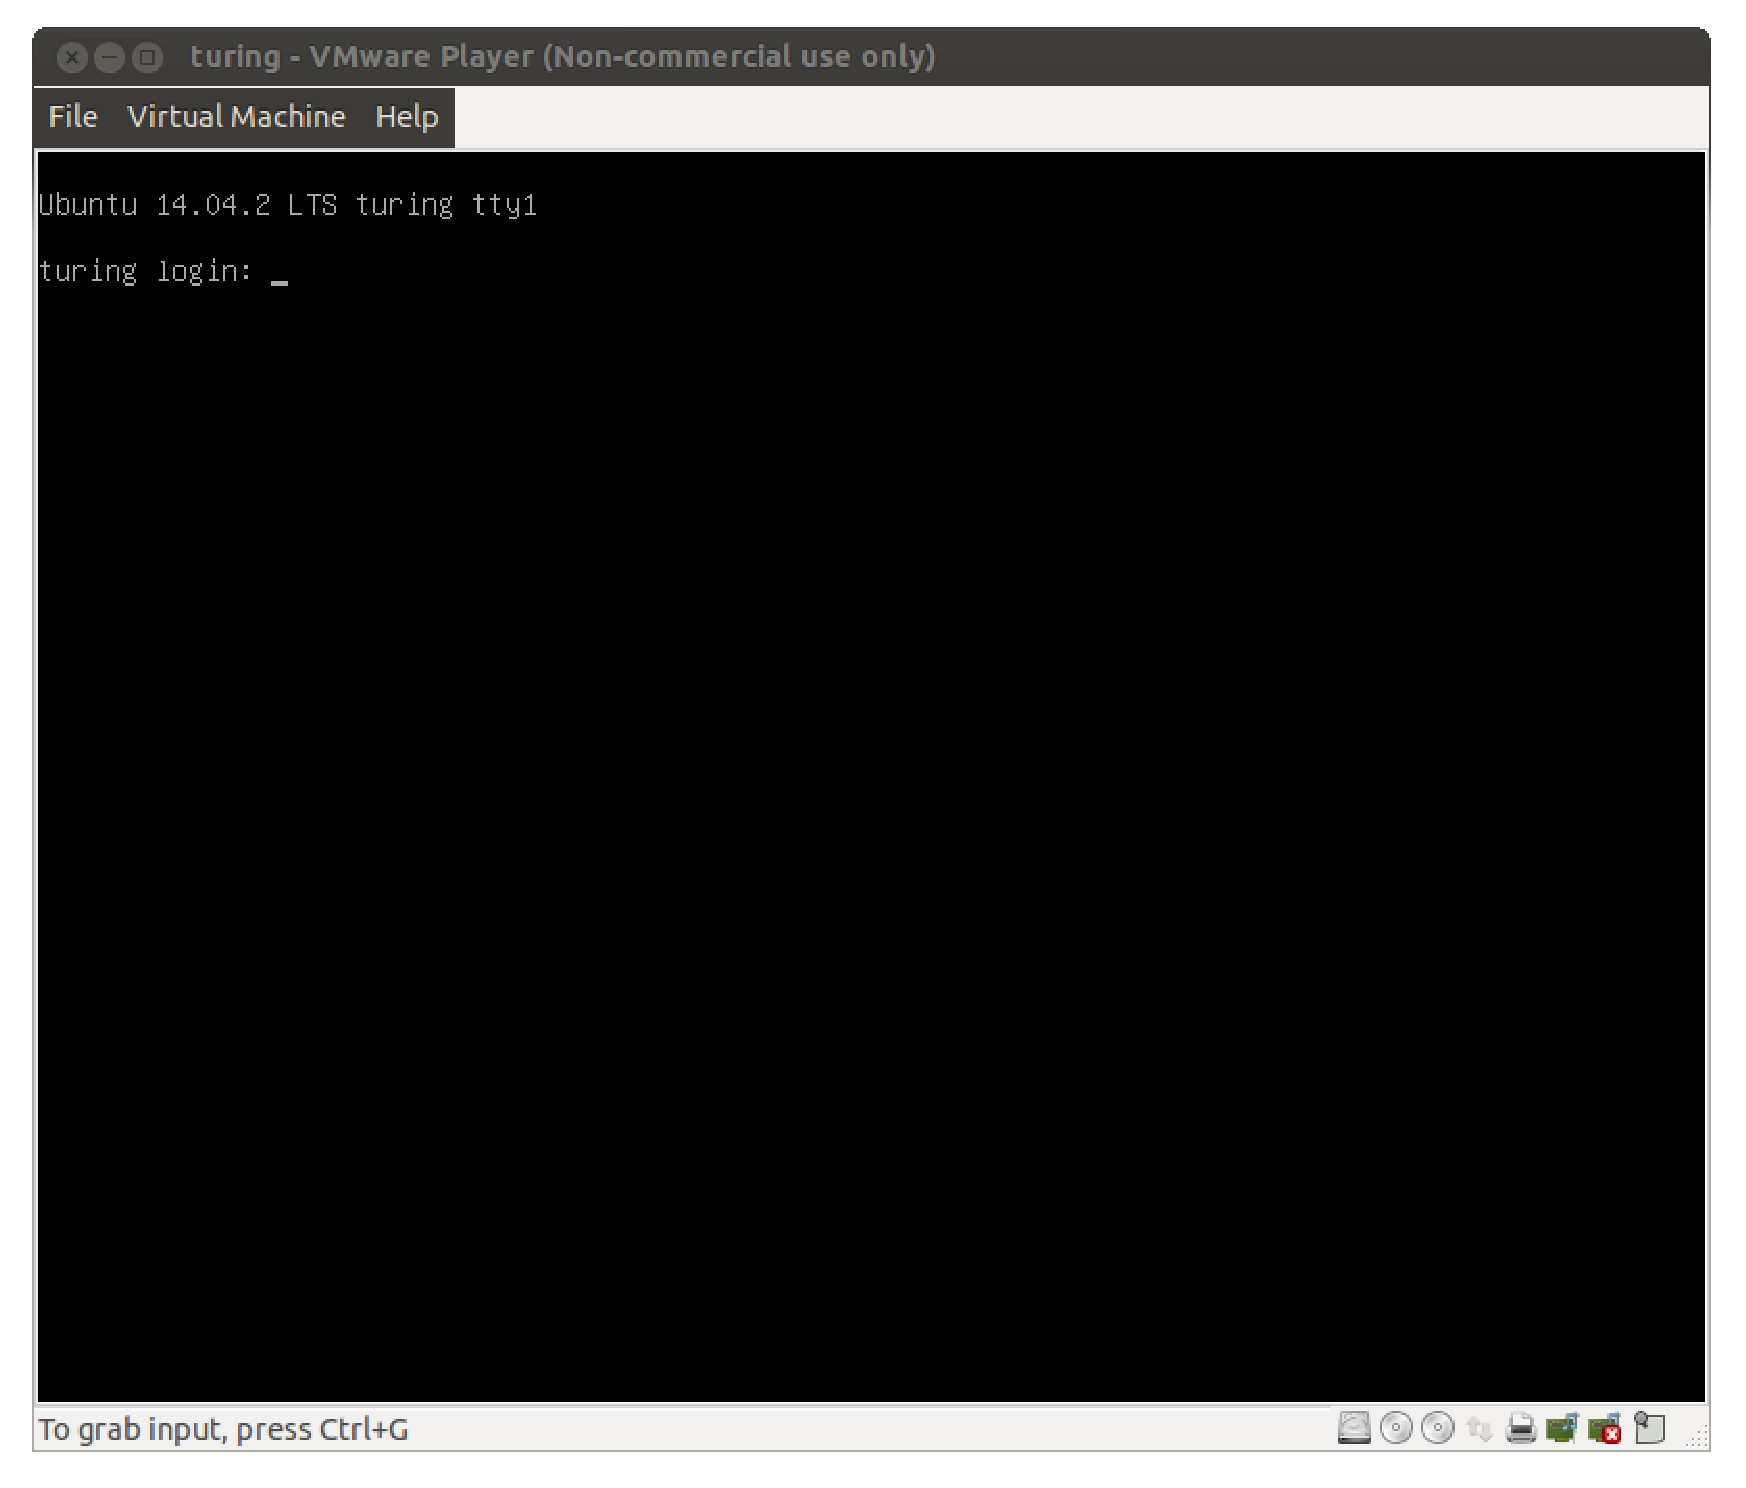
\includegraphics[scale=0.35]{figures/tut1/terminal0.eps}}
      {\caption[\textit{Acesso ao terminal via Ctrl+Alt+F1}]{Login via terminal de texto (acesso com Ctrl+Alt+F1).}\label{tut1:fig:terminal0}}
  \end{figure}

%%%%%%%%%%%%%%%%%%%%%%%%%%% FIM DA FIGURA DO FILE SYSTEM %%%%%%%%%%%%%%%%%%%%%%%%%%%

A segunda forma é usar um ``emulador de terminal'', isto é, dentro do modo gráfico, abre-se um programa que funciona com linha de comando. Na instalação disponibilizada no curso, o terminal está disponível na barra de ferramentas lateral (veja Figura \ref{tut1:fig:terminal1}). De forma geral, em Ubuntu 14.4.02 LTS, você pode acessar o terminal via Painel inicial (também na barra de ferramentas lateral) digitanto o termo ``terminal'' (veja Figura \ref{tut1:fig:terminal2}).\\

%%%%%%%%%%%%%%%%%%%%%%%%%%% FIGURA DO TERMINAL 1 %%%%%%%%%%%%%%%%%%%%%%%%%%%
%  \vspace{-1em}
  \begin{figure}[H]
    %\ffigbox[\FBwidth]
      {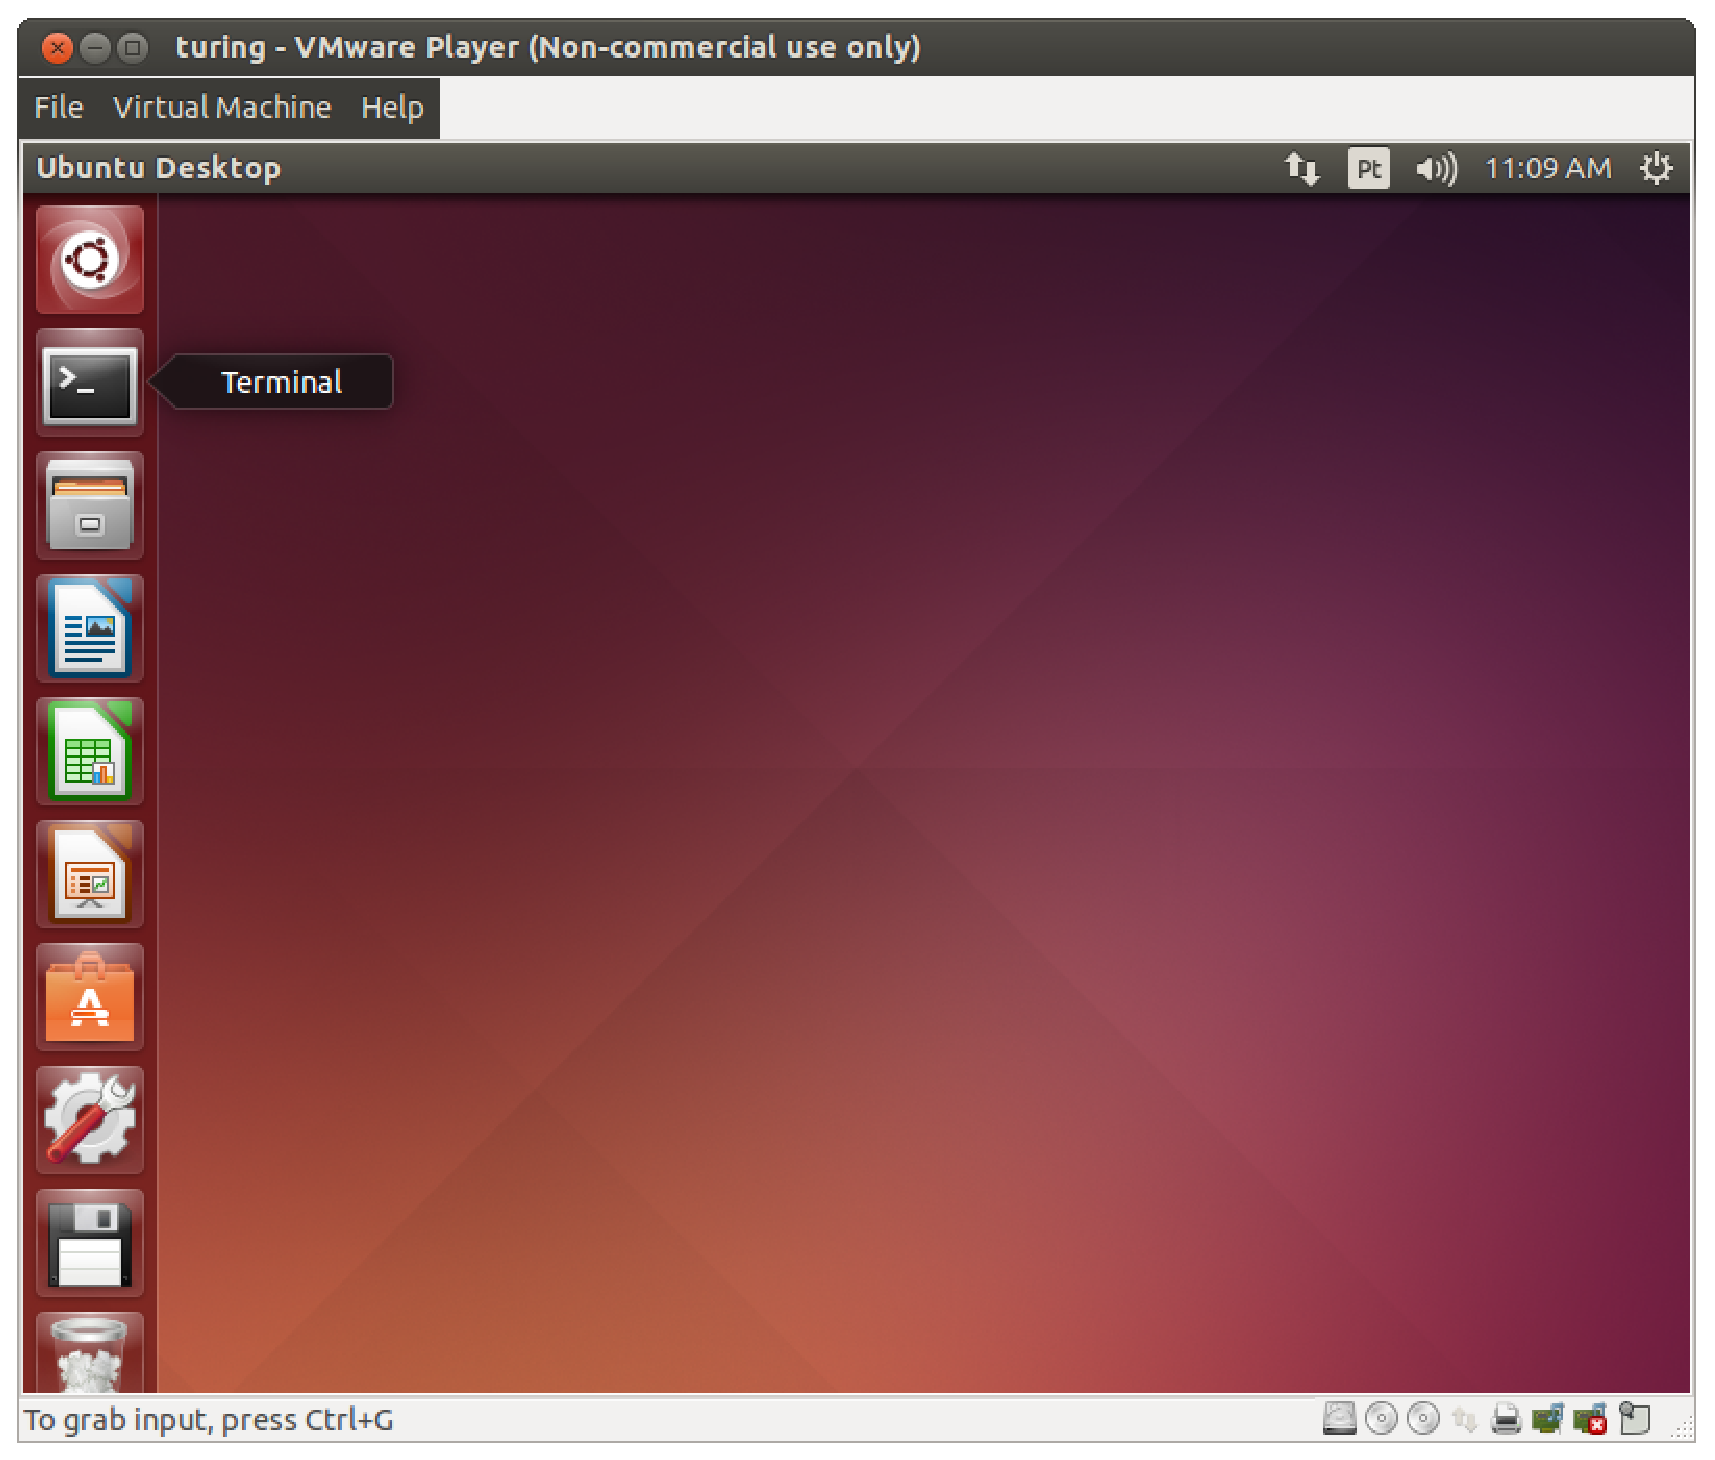
\includegraphics[scale=0.35]{figures/tut1/terminal1.eps}}
      {\caption[\textit{Acesso ao terminal via interface gráfica GNOME}]{Acesso ao terminal via interface gráfica GNOME na barra de ferramentas lateral.}\label{tut1:fig:terminal1}}
  \end{figure}

%%%%%%%%%%%%%%%%%%%%%%%%%%% FIM DA FIGURA DO FILE SYSTEM %%%%%%%%%%%%%%%%%%%%%%%%%%%

%%%%%%%%%%%%%%%%%%%%%%%%%%% FIGURA DO TERMINAL 2 %%%%%%%%%%%%%%%%%%%%%%%%%%%
%  \vspace{-1em}
  \begin{figure}[H]
    %\ffigbox[\FBwidth]
      {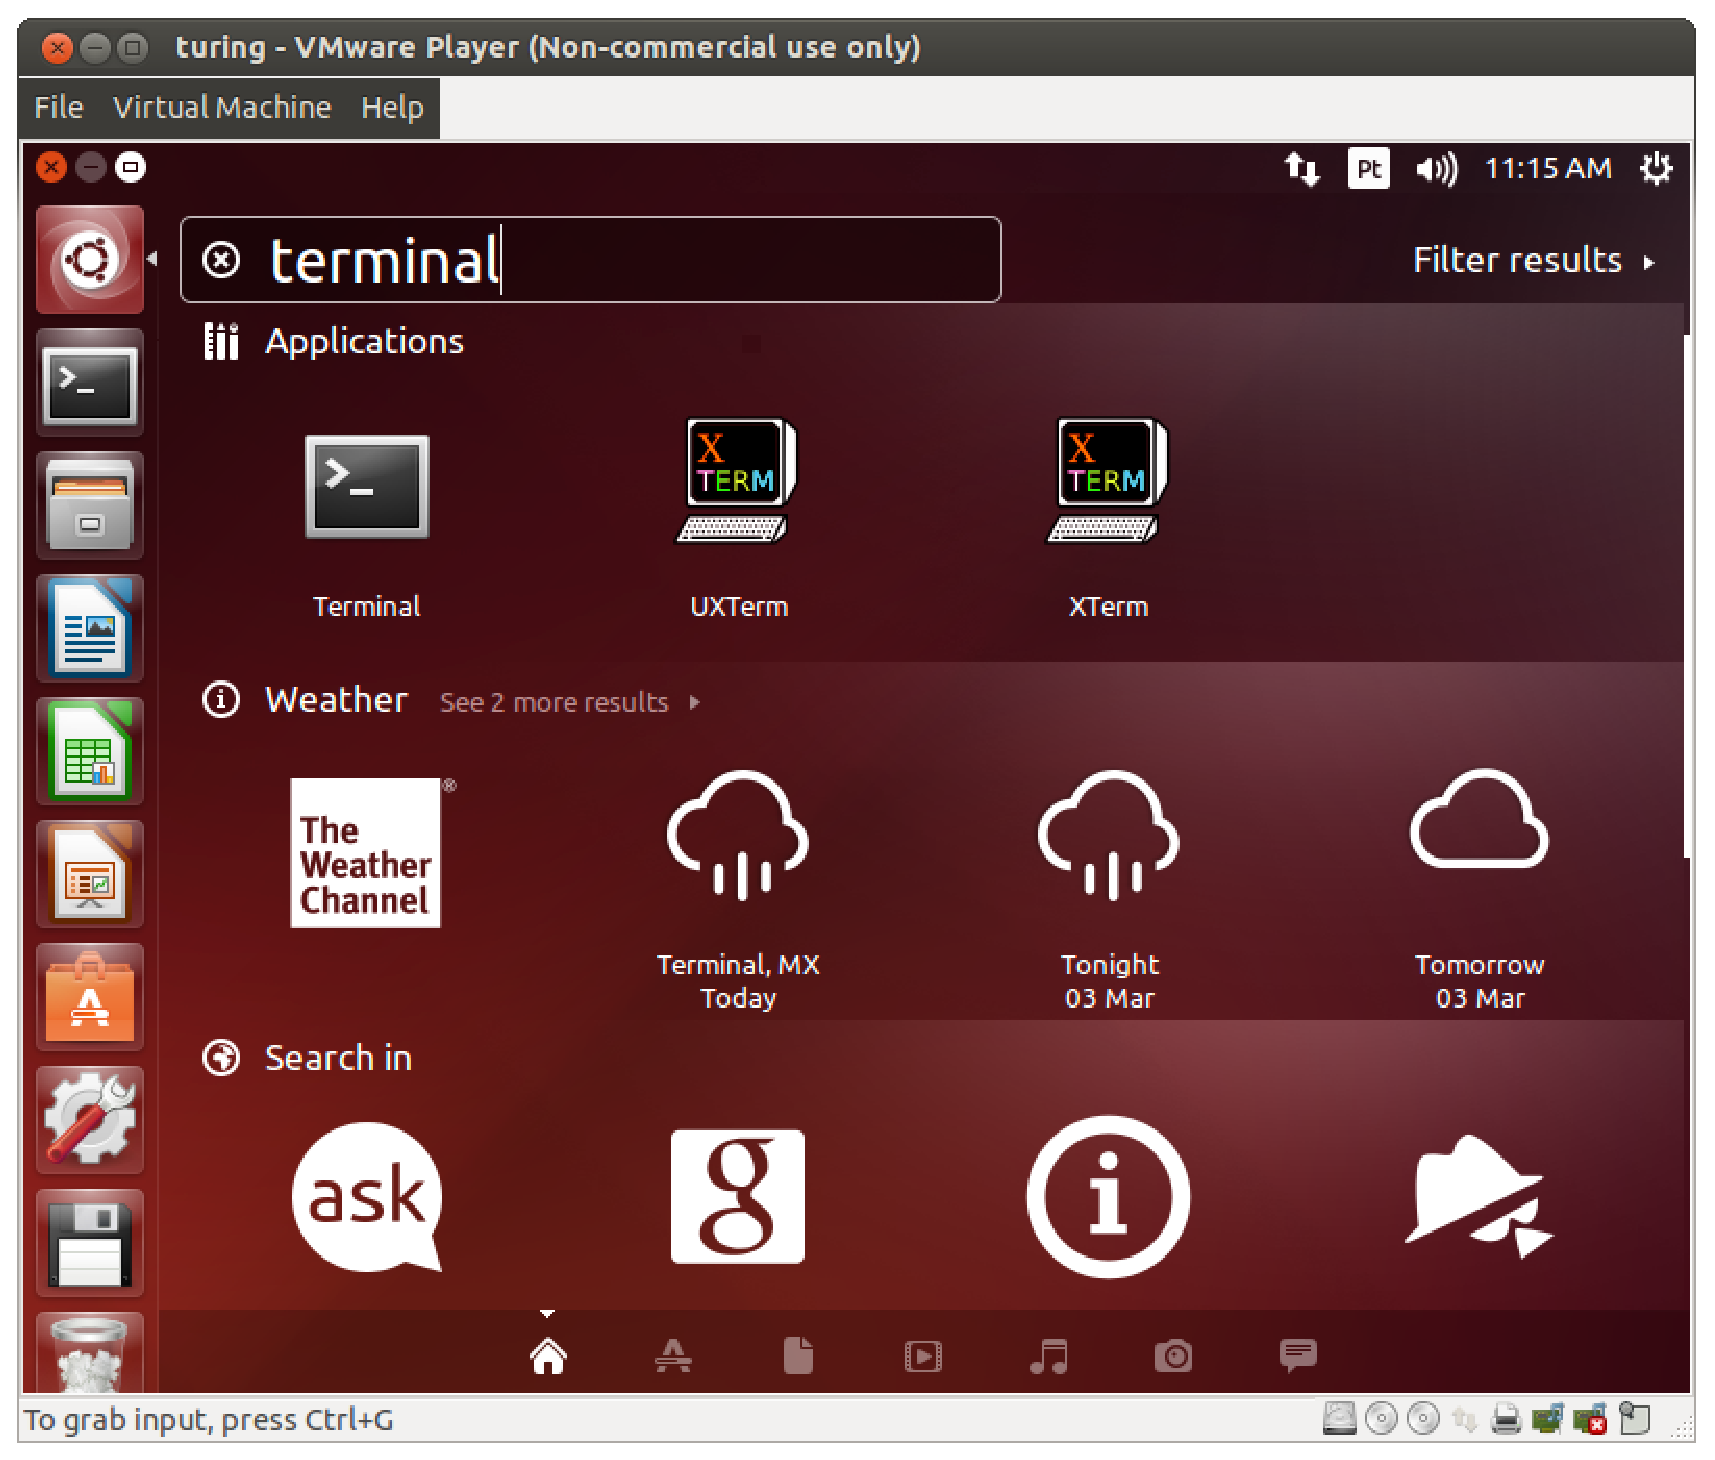
\includegraphics[scale=0.35]{figures/tut1/terminal2.eps}}
      {\caption[\textit{Acesso ao terminal via interface gráfica GNOME usando o Painel incial}]{Acesso ao terminal via interface gráfica GNOME na barra de ferramentas lateral  usando o Painel incial.}\label{tut1:fig:terminal2}}
  \end{figure}

%%%%%%%%%%%%%%%%%%%%%%%%%%% FIM DA FIGURA DO FILE SYSTEM %%%%%%%%%%%%%%%%%%%%%%%%%%%

\subsection{Shell:}\label{tut1:text_mode:commands:shell}
 De qualquer uma das duas formas, o que você verá rodando (após logar-se ou acessar o Terminal) é um programa chamado shell, que é um interpretador de comandos.\\
 \subsection{BASH:}\label{tut1:text_mode:commands:bash}
O BASH (Bourne Again Shell) é o shell desenvolvido para o projeto GNU, da \textit{Free Software Foundation}, que se tornou padrão nas várias distribuições Linux (incluindo Ubuntu).\\

%%%%%%%%%%%%%%%%%%%%%%%%%%% FIGURA DO COMMANDOS %%%%%%%%%%%%%%%%%%%%%%%%%%%
%  \vspace{-1em}
  \begin{figure}[H]
    %\ffigbox[\FBwidth]
      {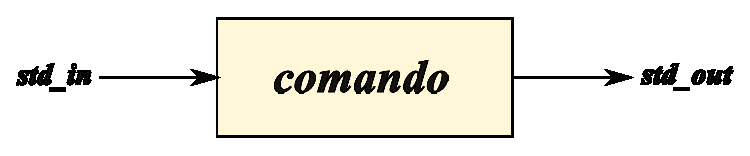
\includegraphics[scale=0.8]{figures/tut1/command_structure.eps}}
      {\caption[\textit{Estrutura de comandos}]{Estrutura de comandos\: \textit{std\_in} representa \textit{standard input}, informações de entrada para o comando;  \textit{std\_out} representa \textit{standard output}, resultado do processamento feito pelo comando.}\label{tut1:fig:commands}}

  \end{figure}

%%%%%%%%%%%%%%%%%%%%%%%%%%% FIM DA FIGURA DO COMANDO %%%%%%%%%%%%%%%%%%

\subsection{Comandos:}\label{tut1:text_mode:commands:commands}
 Nesta seção, examinaremos alguns comandos simples do BASH. É importante que você saiba que não é preciso decorar os comandos apresentados. Para aprendê-los de fato, você deve ir praticando com os exercícios propostos e conforme a sua necessidade.\\
%
Uma noção sobre comandos é importante. Comandos executam tarefas. Não existe comando que não faça nada! Para executar tarefas, comandos necessitam de material para executar a tarefa para o qual ele foi concebido. Esse ``material'' é informação, dados. O comando pegará essa informação e retornará o resultado do processamento, ou seja, o resultado de seu trabalho. Veja a representação desses conceitos na Figura \ref{tut1:fig:commands}. Todo comando requer implicita ou explicitamente uma informação de entrada, \textit{stardard input}, que será processada e exibida como resultado, \textit{stardard input}, na tela ou redireciona a um arquivo (veja Seção \ref{tut1:pipered} abaixo). Guarde esta estrutura, ela será fundamental para você entender o conceito de \textsc{pipes} no final deste tutorial (Seção \ref{tut1:pipered:pipe})\\
%
\subsubsection{Prompt:}\label{tut1:text_modeommands:prompt}
O prompt do BASH tem a seguinte aparência:\\
\indent\indent\userprompt{ }\\
\\
 No caso de \userprompt{ } \textbf{alan} é o nome do usuário, \textbf{turing} é o nome da máquina, ``\textbf{$\sim$}'' é o diretório em que o usuário se encontra, neste caso, ``\textbf{$\sim$}'' representa o diretório \textbf{home} do usuário, e o ``\textbf{\$}'' é o símbolo do tipo de usuário (nesse caso, um usuário normal). Se fosse o usuário root (administrador do sistema), o símbolo seria ``\textbf{\#}''.\\

\subsubsection{Sintaxe dos comandos:}\label{tut1:text_mode:commands:syntax}
É importante lembrar que a linha de comando é \textit{case sensitive}, isto é, diferencia letras maiúsculas de minúsculas. Portanto, ``echo'' é diferente de ``Echo'', que são diferentes de ``ECHO''. Isso também vale para nomes de diretórios e arquivos. Os comandos são, em geral, em letras minúsculas. Muitos deles aceitam argumentos. Os argumentos que começam com um (ou dois) ``-'' são opções. Por exemplo:\\

 \shellcmd{comando -opção1 -opção2 -opção3 argumento}
\\

 Quando os argumentos forem arquivos ou diretórios, tanto o caminho absoluto como o relativo poderão ser usados. Esta linha de comando assume a priori que se algum arquivo faz parte dos argumentos, ele está no seu diretório de trabalho.\\
Outro ponto importante é que você pode digitar os comandos e nomes de arquivos ou diretórios pela metade e depois pressionar ``Tab''. O shell ``tentará completar'' o que falta para você. Se houver mais de uma opção para completar o que foi digitado, as alternativas possíveis serão mostradas. Este é um recurso que facilita muito o uso da linha de comando. Vamos então aos comandos, você deverá abrir um terminal para que faça alguns dos exercícios.\\

\subsubsection{pwd (print working directory):}\label{tut1:text_mode:commands:pwd}
 Mostra o nome e o caminho do diretório atual, ou seja, diretório em que o usuário está, o diretório de trabalho.\\
	\shellcmd{pwd}

	\shellcmd{/home/alan}
\\
\subsubsection{ls (list):}\label{tut1:text_mode:commands:ls}
 Lista os arquivos e subdiretórios de um ou mais diretórios.\\
 \textit{Sintaxe básica:}\\
 \shellcmd{ls [opções] [diretório1] [diretório2] ...}
\\
 \textit{Exemplos:}
\begin {myindentpar}{0.5cm}
\begin{enumerate}[\itshape i.]
  \item {O comando abaixo lista os diretórios e arquivos do /:}\\
  \shellcmd{ls /}

  \item {O comando abaixo lista os diretórios e arquivos do /etc:}\\
  \shellcmd{ls /etc}

   \item {Para listar o conteúdo do / e do /etc, de uma só vez, use:}\\
\shellcmd{ls / /etc}
\\

\stepcounter{ex}
\begin{blackBlock}{\textbf{Exercício 1.\arabic{ex}}}\label{tut1:ex:1.\arabic{ex}}

Liste o conteúdo do diretório /tmp.\\
 Para listar o conteúdo do diretório atual, basta digitar apenas ``ls''. Se o usuário estiver em seu diretório home e digitar ls, a saída será os arquivos e diretórios contidos no /home/alan.\\

\end{blackBlock}

Suponha ainda que o usuário encontra-se em seu diretório home. Existe, dentro do home do usuário, um diretório chamado ``Documentos''. Se quisermos listar o conteúdo deste, podemos usar o comando\\
 \shellcmd{ls /home/alan/Desktop}\\
 mas também podemos usar o caminho relativo (lembra-se?):\\
 \shellcmd{ls Desktop}
\\
 \textit{Opções:}
        \subitem{\textbf{-a} (ou all):} Lista todos os arquivos e diretórios, incluindo os ocultos. No GNU/Linux, os arquivos e diretórios ocultos começam por ``.''. Quando usamos o comando ls como anteriormente (sem nenhuma opção), esses arquivos não são listados.\\
 \textit{Exemplo:}\\
 O comando abaixo listará todos os arquivos e diretórios contidos no barra, incluindo os ocultos.\\
 \userprompt{ls -a}\\

\stepcounter{ex}
\begin{blackBlock}{\textbf{Exercício 1.\arabic{ex}}}\label{tut1:ex:1.\arabic{ex}}

Liste todo o conteúdo do seu diretório home, incluindo os itens ocultos. (Quando fizer isso, você notará que dois itens ``estranhos'' foram listados: o ``.'' e o ``..''. Eles representam, respectivamente, o diretório atual e o diretório acima. Se você estiver em seu diretório home e usar o comando ``ls ../'', o conteúdo do /home será listado).\\

\end{blackBlock}


        \subitem{\textbf{-R:}} Lista o conteúdo de um diretório e dos subdiretórios, recursivamente. Quando você utiliza o comando ls, os arquivos e diretórios contidos num determinado diretório são mostrados. Usando a opção -R, serão listados os arquivos contidos num determinado diretório, e para cada subdiretório também serão listados os arquivos e diretórios nele contidos. E para cada um desses diretórios, também será listado todo o seu conteúdo e assim sucessivamente. Se você usasse ``ls -R /'', o conteúdo de todos os diretórios seria mostrado (não execute esse comando, pois o \textit{output} é longo, ele está aqui apenas para que você entenda o que faz esta opção).\\
         \subitem{\textbf{-l:}} Usa o formato longo para listagem, o que significa que serão listados detalhes sobre cada arquivo e diretório mostrado. Vamos examinar que detalhes são estes. O comando \\
 \shellcmd{ls -l /}\\
imprime:
\\
\indent\indent\texttt{total 44\\
drwxr-xr-x 2 alan alan 4096 Mar  2 11:07 Desktop\\
drwxr-xr-x 2 alan alan 4096 Feb 27 08:25 Documents\\
drwxr-xr-x 2 alan alan 4096 Feb 27 08:25 Downloads\\
-rw-r--r-- 1 alan alan 8980 Feb 27 03:59 examples.desktop\\
drwxr-xr-x 2 alan alan 4096 Feb 27 08:25 Music\\
drwxr-xr-x 2 alan alan 4096 Feb 27 08:25 Pictures\\
drwxr-xr-x 2 alan alan 4096 Feb 27 08:25 Public\\
drwxr-xr-x 2 alan alan 4096 Feb 27 08:25 Templates\\
drwxr-xr-x 2 alan alan 4096 Feb 27 08:25 Videos}\\
 \textit{Permissões:}

 A primeira letra (d) indica que ``Desktop'' é um diretório. Se fosse um arquivo normal, teríamos um ``-'' no lugar (é o caso de examples.desktop). Os próximos nove caracteres representam as permissões do diretório. As permissões de um arquivo ou diretório são r, w e x, apresentadas anteriormente (lembra-se? Leitura, escrita e execução).\\
Para cada três caracteres são mostradas as permissões para um tipo de usuário. Os três primeiros caracteres, no caso ``rwx'', indicam as permissões para o dono do arquivo. A interpretação desta trinca é que o dono do arquivo (no caso, o usuário ``alan''), possui as três permissões sobre o diretório (leitura, escrita e execução). Os três próximos caracteres mostram as permissões para o grupo: ``r-x'', o que significa que o grupo possui permissão de leitura e execução, mas não possui permissão de escrita (há um ``-'' no lugar do ``w'' de escrita). Por último, temos a permissão para os demais usuários do sistema (``r-x'' permissão de leitura e execução).\\

 \textbf{Número de subdiretórios:}

O número da segunda coluna representa o número de subdiretórios contidos. Se for um arquivo comum, esse número será 1.\\

 \textbf{Dono do arquivo:}

A terceira coluna representa o dono do arquivo, que, como dito anteriormente, é o usuário que criou o arquivo ou diretório.\\

 \textbf{Grupo:}

O grupo ao qual o arquivo pertence está mostrado na quarta coluna.\\

 \textbf{Tamanho:}

A coluna seguinte mostra o tamanho do arquivo em bytes. No caso de um diretório, não é mostrado o tamanho total, isto é, considerando todo o conteúdo do diretório, mas sim o tamanho da estrutura diretório, isto é, ainda que seja criado um diretório vazio, ele ocupará 4096 bytes de espaço em disco.\\
Como último comentário sobre este comando, vale dizer que é possível usar mais de uma opção de cada vez. Aliás, isso vale para todo comando. O comando a seguir lista todos os diretórios e arquivos do ``\textbf{/}'', incluindo os ocultos, usando o formato longo de listagem.
\\
 \shellcmd{ls -a -l /}\\
 Também é possível fazer isso da seguinte forma:\\
 \shellcmd{ls -al /}
\\
\stepcounter{ex}
\begin{blackBlock}{\textbf{Exercício 1.\arabic{ex}}}\label{tut1:ex:1.\arabic{ex}}

Liste os arquivos e diretórios do seu diretório \texttt{home/}, incluindo os ocultos e o conteúdo dos subdiretórios.

\end{blackBlock}

\end{enumerate}
\end{myindentpar}


\subsubsection{cd (change directory):}\label{tut1:text_mode:commands:cd}

Entra em (ou muda para) um diretório.

\textit{Sintaxe básica:}

 \shellcmd{cd [diretório]}

\textit{Exemplos:}
\begin {myindentpar}{0.5cm}
\begin{enumerate}[\itshape i.]

\item{Para entrar no diretório root, use:}

  \shellcmd{cd /}
\item{Para entrar no diretório /tmp, basta usar o seguinte comando:}

  \shellcmd{cd /tmp}
\item{Para subir um diretório acima, use:}

 \shellcmd{cd ..}
\item{Para voltar ao diretório imediatamente anteriormente acessado, basta usar:}

 \shellcmd{cd -}

\end{enumerate}
\end{myindentpar}

\stepcounter{ex}
\begin{blackBlock}{\textbf{Exercício 1.\arabic{ex}}}\label{tut1:ex:1.\arabic{ex}}

\begin {myindentpar}{0.5cm}
\begin{enumerate}[\itshape i.]

\item{Entre no diretório home do seu usuário (``/home/alan''). Agora use o seguinte comando:}

 \shellcmd{cd ../../}

\item{Use outro comando para descobrir em que diretório você acabou de entrar.}\\
\item{O que acontece se você digitar apenas o comando ``cd'', sem nenhum argumento?}\\

\end{enumerate}
\end{myindentpar}

\end{blackBlock}

\subsubsection{mkdir (make directory):}\label{tut1:text_mode:commands:mkdir}


 Cria novos diretórios (vazios).\\

 \textit{Sintaxe básica:}

 \shellcmd{mkdir [caminho1/diretório1] [caminho2/diretório2] ...}

\textit{Exemplos:}
 \begin {myindentpar}{0.5cm}
 \begin{enumerate}[\itshape i.]
 \item{Para criar os diretórios ``pasta1'' e ``pasta2'' dentro do diretório /tmp, fazemos:}

 \shellcmd{mkdir /tmp/pasta1 /tmp/pasta2}\\
Naturalmente, se estivéssemos dentro do diretório /tmp, não seria necessário usar o caminho absoluto.\\
Execute:\\
 \userprompt{cd /tmp}\\
e\\
 \userprompt{pwd}\\
o retorno deverá ser:\\
 \texttt{/tmp}\\
Neste caso faríamos:\\
 \shellcmd{mkdir pasta1 pasta2}
\end{enumerate}
\end{myindentpar}

\subsubsection{rmdir (remove directory):}\label{tut1:text_mode:commands:rmdir}

 Remove um ou mais diretórios vazios.

 \textit{Sintaxe básica:}

 \shellcmd{rmdir [caminho1/diretório1] [caminho2/diretório2] ...}

\textit{Exemplos:}
\begin {myindentpar}{0.5cm}
\begin{enumerate}[\itshape i.]

 \item{Para remover os diretórios ``pasta1'' e ``pasta2'' criados como nos exemplos do comando mkdir, poderíamos usar:}

 \shellcmd{rmdir /tmp/pasta1 /tmp/pasta2}

\end{enumerate}
\end{myindentpar}

\stepcounter{ex}
\begin{blackBlock}{\textbf{Exercício 1.\arabic{ex}}}\label{tut1:ex:1.\arabic{ex}}

\begin {myindentpar}{0.5cm}
\begin{enumerate}[\itshape i.]
 \item{Vá até seu diretório home e crie um diretório chamado ``teste''. Use o comando ls para ver que o diretório foi criado. Remova o diretório criado e use novamente o comando ls para ver que a pasta foi removida.}
\end{enumerate}
\end{myindentpar}

\end{blackBlock}

\subsubsection{touch:}\label{tut1:text_mode:commands:touch}

 Pode ser usado para criar novos arquivos vazios e também para mudar a data e a hora de criação de arquivos existentes.
\\
\textit{Sintaxe básica:}

 \shellcmd{touch [opções] [arquivo1] [arquivo2] ...}

\textit{Exemplos:}
 \begin {myindentpar}{0.5cm}
 \begin{enumerate}[\itshape i.]

 \item{Para criar um arquivo vazio chamado ``arquivo\_novo'' no diretório atual, poderíamos usar:}

 \shellcmd{touch arquivo\_novo}
 
 \end{enumerate}
 \end{myindentpar}

\textit{Opções:}
 \begin {myindentpar}{0.5cm}
 \begin{enumerate}[\itshape i.]

 \item{-t [[YY]YY]MMDDhhmm[.ss] - } Altera a data e hora do arquivo para o ano YYYY (nesse caso, pode-se usar os quatro dígitos ou apenas dois), para o mês MM, para o dia DD, para a hora hh, para o minuto mm e para o segundo ss. Lembrando que as opções de ano e segundo são opcionais (por isso foram colocadas entre colchetes).

 \item{Para alterar a data do arquivo ``arquivo\_novo'' para o dia 16/11 (16 de novembro), e o horário para 16h11min, usamos:}

 \shellcmd{touch -t 11161611 arquivo\_novo}
 \item{Suponhamos que quiséssemos alterar os segundos também (para 11, por exemplo):}

 \shellcmd{touch -t 11161611.11 arquivo\_novo}
 \item{Por fim, se quiséssemos que a data do arquivo ``arquivo\_novo'' fosse 18/02/2014, com horário 0h0min, rodaríamos o comando da seguinte forma:}

 \shellcmd{touch -t 201301010000 arquivo\_novo}

 \end{enumerate}
 \end{myindentpar}

\stepcounter{ex}
\begin{blackBlock}{\textbf{Exercício 1.\arabic{ex}}}\label{tut1:ex:1.\arabic{ex}}

 \begin {myindentpar}{0.5cm}
 \begin{enumerate}[\itshape i.]
  \item{Qual é a diferença entre o resultado produzido pelos dois comandos a seguir?}
\\
	\shellcmd{touch ``arquivo\_novo''}\\
e\\
	\shellcmd{touch arquivo\_novo}

 \item{Crie um arquivo chamado ``teste'' em seu diretório home, usando o comando touch. Use ls (com a opção -l) para ver a data do novo arquivo criado. Mude a data e o horário do arquivo para o seu nascimento e use o comando ls para ver a nova data do arquivo.}

 \end{enumerate}
 \end{myindentpar}

\end{blackBlock}

\subsubsection{rm (remove):}\label{tut1:text_mode:commands:rm}
Remove arquivos e diretórios.\\
 \textit{Sintaxe básica:}
\\
\shellcmd{rm [opções] [arquivo1] [arquivo2] ...}

\textit{Exemplos:}
\begin {myindentpar}{0.5cm}
\begin{enumerate}[\itshape i.]

\item{Criamos um arquivo chamado ``teste'' no diretório /tmp:}\\
 \shellcmd{touch /tmp/teste}

\item{Agora vamos removê-lo:}\\
 \shellcmd{rm /tmp/teste}

\end{enumerate}
\end{myindentpar}

\textit{Opções:}

\textbf{-r:} Opção usada para remover recursivamente diretórios e seu conteúdo. Pode ser usada também para remover diretórios vazios.\\

\textit{Exemplos:}
\begin {myindentpar}{0.5cm}
\begin{enumerate}[\itshape i.]

 \item{Vamos criar um diretório (vazio) chamado ``pasta''.}\\
	\shellcmd{mkdir pasta}\\
 \item{Se usarmos o seguinte comando para removê-lo, veremos um erro e o diretório não será removido:}\\
	\shellcmd{rm pasta}\\
o terminal imprime:\\
\texttt{rm: não foi possível remover “pasta”: É um diretório}

Para removê-lo, teríamos que executar o comando:

 \shellcmd{rm -r pasta}\\
Poderíamos também usar o comando \texttt{rmdir} já apresentado.\\

 \item{Vamos criar agora um diretório chamado ``pasta\_teste'' dentro do diretório /tmp. E dentro de ``pasta\_teste'', isto é, no /tmp/pasta\_teste, vamos criar um arquivo chamado ``arquivo\_teste''. Depois vamos removê-los.}
\\
 \shellcmd{mkdir /tmp/pasta\_teste}\\
 \shellcmd{touch /tmp/pasta\_teste/arquivo\_teste}

Para remover, poderíamos fazer da seguinte maneira:\\
 \shellcmd{rm /tmp/pasta\_teste/arquivo\_teste}\\
 \shellcmd{rmdir /tmp/pasta\_teste}

Mas a opção -r do comando \texttt{rm} nos permite remover o diretório e todo o seu conteúdo. Por isso, o comando a seguir já seria suficiente para remover o diretório ``pasta\_teste'' e seu conteúdo (no caso, o arquivo ``arquivo\_teste'').\\
\shellcmd{rm -r /tmp/pasta\_teste}\\
\textbf{Atenção:} O comando rm é \textbf{definitivo}, ou seja, uma vez que o usuário removeu um arquivo (ou um diretório), este não poderá ser recuperado. Não funciona simplesmente como uma lixeira, mas sim remove definitivamente o que for passado como argumento.\\

\end{enumerate}
\end{myindentpar}

\subsubsection{cp (copy):}\label{tut1:text_mode:commands:cp}

 Este comando serve para copiar arquivos.\\

\textit{Sintaxe básica:}
\\
 \shellcmd{cp [opções] [origem] [destino]}

\textit{Exemplos:}
\begin {myindentpar}{0.5cm}
\begin{enumerate}[\itshape i.]

\item{Para copiar o arquivo ``teste'' do /tmp para o diretório home do usuário:}\\
 \shellcmd{cp /tmp/teste $\sim$}
\end{enumerate}
\end{myindentpar}

\textit{Opções:}

 \textbf{-R:} Copia recursivamente os subdiretórios e seu conteúdo.\\

\textit{Exemplos}
\begin {myindentpar}{0.5cm}
\begin{enumerate}[\itshape i.]

\item{Suponha que um usuário possui um diretório no /tmp (/tmp/diretorio) e quer copiá-lo para seu home. Suponha ainda que esse diretório a ser copiado não está vazio.}\\
 \shellcmd{cd /tmp/diretorio}\\
 \shellcmd{ls}\\
o terminal deverá imprimir:\\
\userprompt{\\}
\texttt{arquivo}
\\
para copiar o diretório e seu conteúdo para o seu home, você deve executar o comando:\\
 \shellcmd{cp -R /tmp/diretorio $\sim$/}

\end{enumerate}
\end{myindentpar}

\subsubsection{mv (move):}\label{tut1:text_mode:commands:mv}

 Move e renomeia arquivos e diretórios.\\

\textit{Sintaxe básica}

 \shellcmd{mv [opções] [origem] [destino]}

\textit{Exemplos:}
\begin {myindentpar}{0.5cm}
\begin{enumerate}[\itshape i.]

\item{Suponha que um usuário possui um arquivo em sua home chamado arquivo1. Para renomear este arquivo para arquivo\_novo, supondo que o usuário está em sua home, bastaria usar:}
\\
 \shellcmd{mv arquivo1 arquivo\_novo}\\
\item{Suponhamos agora que queremos mover o ``arquivo\_novo'' para o diretório /tmp. Para isso, o seguinte comando seria eficaz (estamos supondo ainda que o usuário está em sua home):}
\\
 \shellcmd{mv arquivo\_novo /tmp/}\\
 Após a execução desse comando, ``arquivo\_novo'' estaria no diretório /tmp e não haveria mais uma cópia do arquivo no diretório home do usuário.\\

\end{enumerate}
\end{myindentpar}

\textit{Opções:}

 \textbf{-v, --verbose:} Explica o que está sendo movido.\\

\subsubsection{cat (concatenate):}\label{tut1:text_mode:commands:cat}

 Concatena arquivos e imprime o resultado no terminal.\\

\textit{Sintaxe básica:}

 \shellcmd{cat [arquivo1] [arquivo2] ...}\\
Para ilustrar o uso deste comando, vamos primeiro criar dois arquivos de texto não-vazios. Para isso, abra um editor de texto - pode ser qualquer um, utilizaremos o gedit por ser bastante simples.\\
 Para abrir o gedit, procure-o em seu Painel Inicial (veja Figura \ref{tut1:fig:gedit})

%%%%%%%%%%%%%%%%%%%%%%%%%%% FIGURA PARA ABRIR GEDIT %%%%%%%%%%%%%%%%%%%%%%%%%%%
%  \vspace{-1em}
  \begin{figure}[H]
    %\ffigbox[\FBwidth]
      {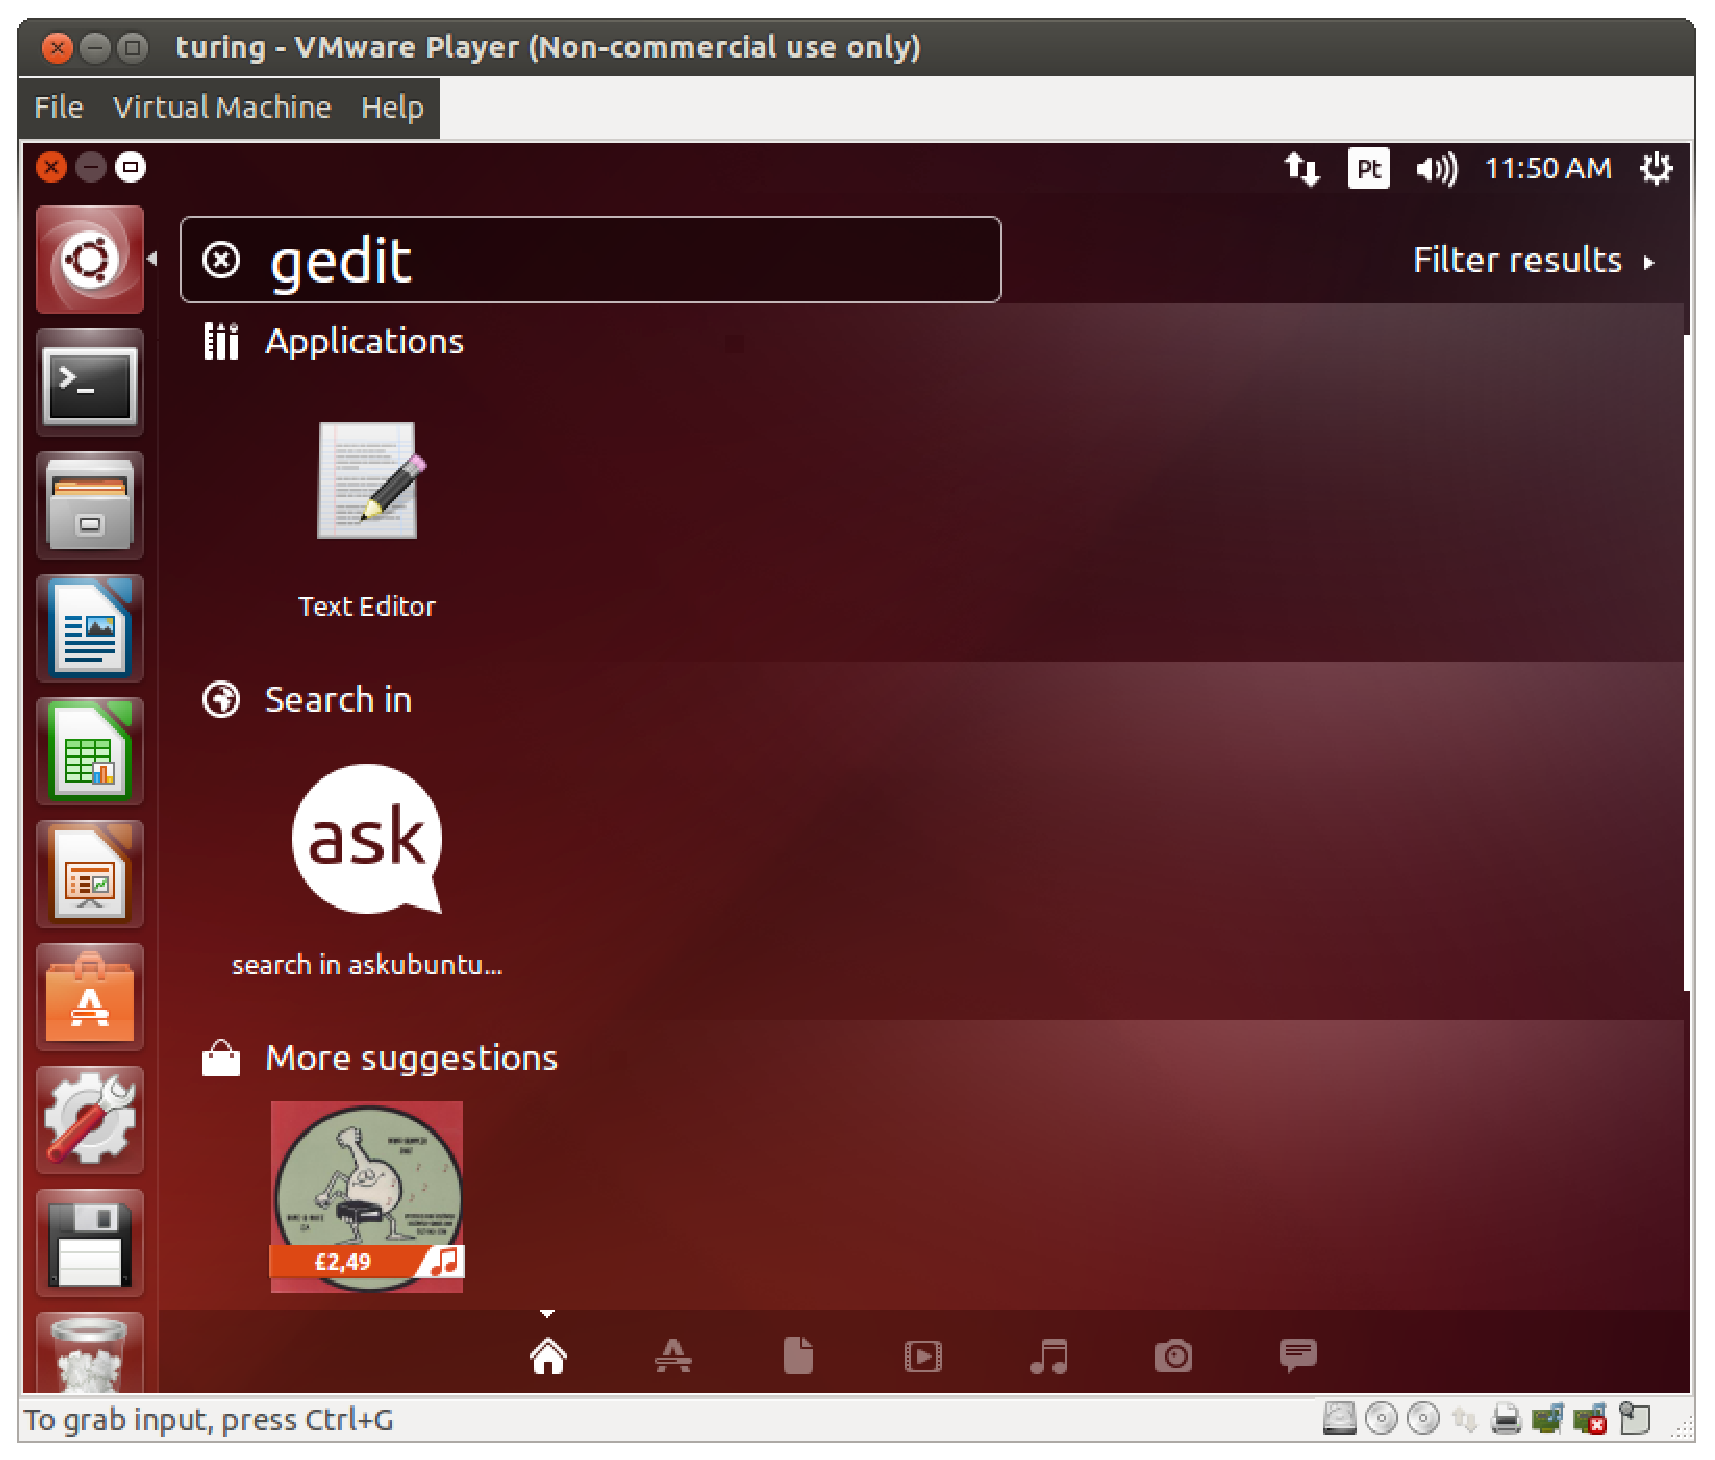
\includegraphics[scale=0.35]{figures/tut1/gedit.eps}}
      {\caption[\textit{Acesso ao gedit via interface gráfica GNOME usando o Painel incial}]{Acesso ao editor de texto gedit via interface gráfica GNOME na barra de ferramentas lateral  usando o Painel incial.}\label{tut1:fig:gedit}}
  \end{figure}

%%%%%%%%%%%%%%%%%%%%%%%%%%% FIM DA FIGURA DO FILE SYSTEM %%%%%%%%%%%%%%%%%%%%%%%%%%%

 Crie dois arquivos (arquivo1.txt e arquivo2.txt\footnote{O termo ``.txt'' é o que chamamos de extensão. Extensões são usadas pelo sistema para reconhecer que tipo de arquivo se trata e qual o aplicativo que potencialmente poderá abrir-lo. Para Linux, isso não faz muita diferença por que a maioria dos arquivos são arquivos texto. De qualquer fora, é boa prática criar arquivos com extensões mesmo que seja somente para sua referência.}), contendo qualquer texto e salve-os no diretório home do usuário.\\
 Observe agora o uso do comando cat:\\
\userprompt{pwd}
\\
o terminal deverá imprimir:\\
\texttt{/home/alan}\\

Verifique o conteúdo do diretório:\\
\userprompt{ls}\\

o terminal deverá imprimir:\\
\texttt{
Desktop    Downloads         Music     Public     Videos\\
Documents  examples.desktop  Pictures  Templates} \\

Verifique o conteúdo do arquivo1.txt:\\
\userprompt{cat arquivo1.txt}
\\
o terminal deverá imprimir:\\
\texttt{arquivo1.txt\\
etc.\\
etc.\\
}
Verifique o conteúdo do arquivo1.txt:\\
\userprompt{cat arquivo2.txt}
\\
o terminal deverá imprimir:\\
\texttt{arquivo2.txt\\
blá\\
blá\\
}
Verifique o conteúdo dos dois arquivos com um único comando:\\
\userprompt{cat arquivo1.txt arquivo2.txt}
\\
o terminal deverá imprimir:\\
\texttt{arquivo1.txt\\
etc.\\
etc.\\
arquivo2.txt\\
blá\\
blá\\
}

\subsubsection{find:}\label{tut1:text_mode:commands:find}

O comando \textit{find} é usado para procurar por diretórios e arquivos no disco. Possui várias opções, mas mostraremos apenas alguns exemplos simples.\\

\textit{Exemplos:}
\begin {myindentpar}{0.5cm}
\begin{enumerate}[\itshape i.]

\item{Este exemplo procura por um arquivo ou diretório com o nome ``Documents'' a partir do / (diretório root):}
\\
 \shellcmd{find / -name Documents}

\item{Este outro procura por um arquivo ou diretório com o nome ``Music'' a partir do diretório home do usuário:}
\\
 \shellcmd{find $\sim$ -name Music}

 É importante salientar que ``a partir do diretório x'' significa que o comando procurará dentre tudo o que estiver contido no tal diretório, incluindo os arquivos e os subdiretórios, bem como seu conteúdo e assim por diante.\\
\end{enumerate}
\end{myindentpar}


\subsubsection{clear:}\label{tut1:text_mode:commands:clear}

 Use o comando clear e descubra o que ele faz:\\
\shellcmd{clear}

\subsubsection{exit:}\label{tut1:text_mode:commands:exit}

 Este comando serve para sair do shell (interpretador) e para efetuar o log out do usuário no terminal.\\
\subsubsection{echo:}\label{tut1:text_mode:commands:echo}

Mostra um texto. Por agora, pode parecer um comando pouco útil, mas é bastante usado sobretudo em scripts para exibir mensagens ao usuário.\\

\textit{Sintaxe básica:}

 \shellcmd{echo mensagem}

\textit{Exemplos:}
\begin {myindentpar}{0.5cm}
\begin{enumerate}[\itshape i.]

 \item{Note que a primeira linha corresponde ao comando, e a segunda, ao resultado da execução deste comando:}

\userprompt{echo mensagem}

o terminal deverá imprimir:\\
\indent\indent\texttt{mensagem}

\end{enumerate}
\end{myindentpar}


\textit{Mais um exemplo:}


\userprompt{echo Uma mensagem mais comprida}

o terminal deverá imprimir:\\
\indent\indent\texttt{Uma mensagem mais comprida}
\\

\stepcounter{ex}
\begin{blackBlock}{\textbf{Exercício 1.\arabic{ex}}}\label{tut1:ex:1.\arabic{ex}}

\begin {myindentpar}{0.5cm}
\begin{enumerate}[\itshape i.]
 \item{Rode o comando a seguir e tenha certeza de que entendeu sua saída.}
\\
 \shellcmd{echo $\sim$}\\
 \item{Rode os comandos a seguir e observe a diferença entre seus resultados.}
\\
 \shellcmd{echo ``aspas''}\\
 \shellcmd{echo ````aspas''''}

\end{enumerate}
\end{myindentpar}


\end{blackBlock}

\subsubsection{date:}\label{tut1:text_mode:commands:date}

 O comando date imprime ou modifica a data e o horário do sistema. é importante salientar que somente o usuário root e usuários privilegiados podem rodar este comando.\\

\textit{Sintaxe básica:}

 \shellcmd{date [data]}

\textit{Exemplos:}
\begin {myindentpar}{0.5cm}
\begin{enumerate}[\itshape i.]

\item{Para visualizar a data e a hora do sistema:}
 \shellcmd{date}\\
 \texttt{Mon Mar  2 12:04:45 PST 2015}\\

\item{Para alterar a data e a hora do sistema, basta usar o comando da seguinte maneira:}

 \shellcmd{date MMDDhhmm[[YYyy][.ss]]}

 Onde MM é o mês, DD é o dia, hh é a hora, mm são os minutos. Opcionalmente, podem ser usados o ano (com 2 ou 4 dígitos) e os segundos (ss). Para alterar a data do sistema para o dia 1 de fevereiro e o horário para 14:30, poderíamos fazer:

 \shellcmd{date 02011430}

\end{enumerate}
\end{myindentpar}

\subsubsection{chmod (change mode):}\label{tut1:text_mode:commands:chmod}

 Este comando é usado para mudar permissões de arquivos ou diretórios.\\

\textit{Sintaxe básica:}

\shellcmd{chmod [permissões] [diretório/arquivo]}\\

Há duas formas de usar o comando.\\
A primeira forma é bem simples. Você precisa saber que ``u'' representa o dono (``user''), ``g'', o grupo, ``o'', os demais usuários e ``a'', por sua vez, representa todos (``all''). As letras ``r'', ``w'' e ``x'' são as permissões apresentadas anteriormente. Além disso, você precisa saber que ``+'' acrescenta uma permissão, ao passo que ``-'' retira. Se usarmos ``='', teremos uma permissão exata. Vamos examinar alguns exemplos para podermos entender melhor.\\

\text{Exemplos:}
\\
Consideremos o arquivo exemplo (aquele que apareceu no comando ls), cuja permissão era rw-r--r--. Consideremos ainda que estamos no diretório home do usuário curso (/home/alan).
 \begin {myindentpar}{0.5cm}
 \begin{enumerate}[\itshape i.]

\item{Suponhamos que queremos acrescentar permissão de escrita ao grupo. Poderíamos fazer isso da seguinte forma:}
\\
 \shellcmd{chmod g+w exemplo}\\
\item{Suponhamos agora que acabamos de nos arrepender e queremos tirar a permissão de escrita para o grupo. Poderíamos fazer da seguinte forma:}
\\
 \shellcmd{chmod g-w exemplo}\\
\item{Para acrescentar a permissão de execução a todos os usuários, fazemos:}
\\
 \shellcmd{chmod a+x exemplo}\\
\item{Para que os demais usuários fiquem sem permissão de leitura, mas tenham permissão de escrita e execução, temos:}
\\
 \shellcmd{chmod o=wx exemplo}\\

O outro modo de alterar permissões é usando o chamado modo octal. Para usá-lo, é preciso ter em mente o seguinte:\\

\indent\textbf{0} - Nenhuma permissão de acesso.\\
\indent\textbf{1} - Permissão de execução.\\
\indent\textbf{2} - Permissão de escrita.\\
\indent\textbf{4} - Permissão de leitura.\\

A partir disso, podemos obter qualquer permissão, somando os números correspondentes às permissões desejadas.\\

\indent\textbf{3} - Permissão de execução e escrita (1 + 2).\\
\indent\textbf{5} - Permissão de execução e leitura (1 + 4).\\
\indent\textbf{6} - Permissão de escrita e leitura (2 + 4).\\
\indent\textbf{7} - Todas as permissões: execução, escrita e leitura (1 + 2 + 4).\\

 Com esses algarismos, construímos números com três dígitos (XYZ, onde X representa a permissão que será definida para o dono, Y, a permissão do grupo, e Z é a permissão para outros usuários). Vamos mostrar como usar o modo octal.\\

\end{enumerate}
\end{myindentpar}

\textit{Exemplos:}
\begin {myindentpar}{0.5cm}
\begin{enumerate}[\itshape i.]

\item{Observe o exemplo a seguir:}

 \shellcmd{chmod 762 arquivo1.txt}\\
ou\\
\shellcmd{chmod 762 /home/alan/arquivo1.txt}

Nesse caso, estamos dando permissão 7 ao dono do arquivo exemplo, isso significa que estamos dando permissão de leitura, escrita e execução ao dono do arquivo. Para o grupo, demos permissão 6 (escrita e leitura). Aos demais, demos apenas permissão de escrita (permissão 2).\\
Vale lembrar que este comando (como outros) aceita caminhos relativos e absolutos.\\
\end{enumerate}
\end{myindentpar}

\stepcounter{ex}
\begin{blackBlock}{\textbf{Exercício 1.\arabic{ex}}}\label{tut1:ex:1.\arabic{ex}}

\begin {myindentpar}{0.5cm}
\begin{enumerate}[\itshape i.]
 \item{Como você daria permissão de escrita e leitura para o dono do arquivo exemplo, permissão de leitura para o grupo e nenhuma permissão para os demais usuários, usando o modo octal?}

 \item{Como você daria permissão de leitura e escrita a todos os usuários usando o primeiro modo apresentado?}

\end{enumerate}
\end{myindentpar}

\end{blackBlock}

\subsubsection{passwd (password):}\label{tut1:text_mode:commands:passwd}

Este comando é usado para atualizar informações dos usuários.\\
Neste módulo, diremos apenas que ele pode ser usado para alterar a senha do seu próprio usuário.\\

\textit{Sintaxe básica:}
\\
 \shellcmd{passwd}\\
Após digitar este comando no terminal, o usuário deverá digitar sua senha atual (lembrando que não haverá nenhuma evidência - como asteriscos ou pontos - de que o usuário está digitando), depois a nova senha e, por último, será pedido para que o usuário confirme a nova senha.\\

\subsubsection{su:}\label{tut1:text_mode:commands:su}

O comando su é usado para mudar de usuário ou para tornar-se superuser (administrador do sistema ou usuário root).\\

\textit{Sintaxe básica:}
\\
 \shellcmd{su [usuário]}

\textit{Exemplos:}
\begin {myindentpar}{0.5cm}
\begin{enumerate}[\itshape i.]

\item{Suponha que você esteja ``logado'' num terminal como ``usuario1'' e deseja logar-se como ``usuario2'', sem ter que encerrar a sessão como ``usuario1'':}
\\
Se você executar:\\
\userprompt{whoami}

o terminal deverá imprimir:\\
\indent\indent\texttt{usuario1}
\\
Se você executar:\\
\userprompt{su usuario2}

o terminal deverá imprimir:\\
\indent\indent\texttt{Senha:}
\\
Se você entrar com a senha e  executar:\\
\userprompt{whoami}

o terminal deverá imprimir:\\
\indent\indent\texttt{usuario2}
\\
para sair deste usuário basta executar:\\
\userprompt{exit}

o terminal deverá imprimir:\\
\texttt{exit}

Se você executar:\\
\userprompt{whoami}

o terminal deverá imprimir:\\
\indent\indent\texttt{usuario1}\\

Acompanhe a sequência de comandos: a princípio, o usuário que estava logado era ``usuario1'', o que pôde ser confirmado pelo comando whoami. A seguir, para mudar sua identidade para ``usuario2'', o comando su foi utilizado - note que foi preciso digitar a senha de usuario2. Depois de autenticado, o usuário logado passou a ser ``usuario2''. Com o comando exit fechou-se a sessão de ``usuario2'' e a identidade voltou a ser ``usuario1''.\\

Para tornar-se o usuário root, basta usar o comando su sem nenhum argumento:
\userprompt{su}

o terminal deverá imprimir:\\
\indent\indent\texttt{senha:}\\
ou\\
\indent\indent\texttt{Password:}\\
Ao inserir a senha, você deverá obter:\\
\indent\indent\texttt{root@vm-ubuntu:/home/alan\#}\\
Note que foi necessário digitar a senha do usuário root.\\
\end{enumerate}
\end{myindentpar}

\subsubsection{sudo (su ``do''):}\label{tut1:text_mode:commands:sudo}
\begin {myindentpar}{0.5cm}
\begin{enumerate}[\itshape i.]

Comando usado para obter privilégios de outros usuários (sobretudo do usuário root) para executar determinadas tarefas.\\

Algumas tarefas como instalar programas, alterar configurações essenciais do sistema etc. não podem ser desempenhadas por qualquer usuário, mas apenas pelo usuário root e/ou por alguns outros usuários que possam utilizar o comando sudo (os chamados sudoers).\\
No Ubuntu 14.04.02, o usuário criado no momento da instalação é um sudoer e não é criada uma senha para usuário root. Isso significa que, para desempenhar tarefas administrativas é necessário acrescentar ``sudo'' à frente do comando.\\
Observe o seguinte exemplo:\\
\userprompt{whoami}

o terminal deverá imprimir:\\
\indent\indent\texttt{alan}

se você tentar executar o seguinte comando:\\
\userprompt{shutdown -h now}

o terminal deverá imprimir:\\
\texttt{shutdown: Precisa ser root}

Se você executar:\\
\userprompt{sudo shutdown -h now}

o terminal deverá imprimir:\\
\indent\indent\texttt{[sudo] password for aluno:}\\

O usuário aluno gostaria de desligar seu computador através da linha de comando, usando o comando shutdown. Acontece que, para executar tal comando, é necessário ser root. Por ser um sudoer, o usuário curso utilizou o comando sudo (observe que foi preciso digitar a senha do usuário curso) e conseguiu desligar o computador.\\
Para anular este comando pressione Ctrl+C.\\

\end{enumerate}
\end{myindentpar}


\subsubsection{wc (word count):}\label{tut1:text_mode:commands:wc}

O comando wc é usado para contar linhas, palavras e bytes de um arquivo ou do que for escrito no terminal.\\

\textit{Sintaxe básica}
\\
 \shellcmd{wc [opções] [arquivo]}  \textit{Opções}

	\indent\indent\textbf{-c:} Imprimir a contagem de bytes.\\
	\indent\indent\textbf{-l:} Imprimir o número de linhas.\\
	\indent\indent\textbf{-w:} Imprimir o número de palavras.\\


\textit{Exemplos:}

Vamos usar, para estes exemplos, o conteúdo dos arquivos ``arquivo1.txt'' e ``arquivo2.txt'', mostrados na explicação do comando cat.  

\begin {myindentpar}{0.5cm}
\begin{enumerate}[\itshape i.]
\item{Para exibir o número de linhas do arquivo ``arquivo1.txt'', usaríamos:}

\shellcmd{wc -l arquivo1.txt}\\
\texttt{3 arquivo1.txt}\\
\item{Para exibir o número de palavras e de bytes do arquivo ``arquivo2.txt'':}

\shellcmd{wc -wc arquivo2.txt}\\
\texttt{2 22 arquivo2.txt}\\
\item{Se usássemos o comando wc sem nenhuma opção para ``arquivo1.txt'', obteríamos:}

\shellcmd{wc arquivo1.txt}\\
\texttt{3 3 19 arquivo1.txt}\\

onde o primeiro número é a contagem de linhas, o segundo, de palavras, e o terceiro, o de bytes.\\

\end{enumerate}
\end{myindentpar}

\section{Comandos concatenados e redirecionamento}\label{tut1:pipered}

Além dos comandos apresentados anteriormente, a linha de comando ainda possui outros recursos para facilitar tarefas. Nesta seção, apresentaremos algumas ferramentas de direcionamento de entrada e saída.\\

\subsection{Comandos concatenados via pipe (``|''):}\label{tut1:pipered:pipe}

%%%%%%%%%%%%%%%%%%%%%%%%%%% FIGURA DO COMMANDO COM PIPE %%%%%%%%%%%%%%%%%%%%%%%%%%%
%  \vspace{-1em}
  \begin{figure}[H]
    %\ffigbox[\FBwidth]
      {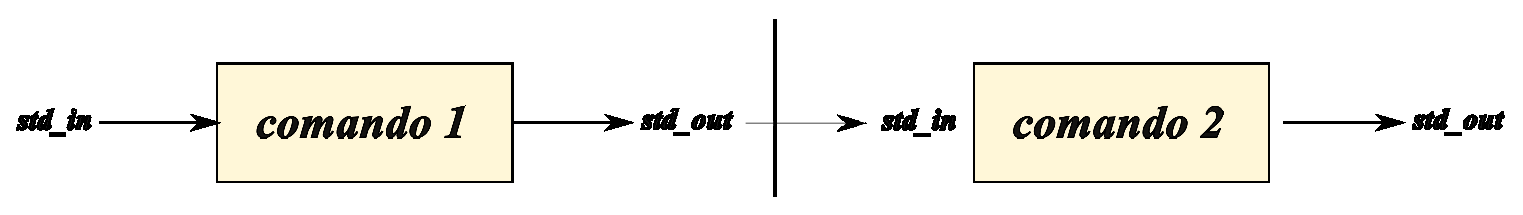
\includegraphics[scale=0.6]{figures/tut1/pipe.eps}}
      {\caption[\textit{Estrutura de comandos utilizando pipe}]{Estrutura de comandos 1 e 2 concatenados com o \textsc{pipe}\: \textit{std\_in} representa \textit{standard input}, informações de entrada para o comando;  \textit{std\_out} representa \textit{standard output}, resultado do processamento feito pelo comando.}\label{tut1:fig:pipe}}

  \end{figure}

%%%%%%%%%%%%%%%%%%%%%%%%%%% FIM DA FIGURA DO COMANDO  COM PIPE %%%%%%%%%%%%%%%%%%

O pipe (|) é usado para fazer encadeamento de processos. Lembre-se da estrutura dos comandos, eles requerem um \textit{stardard input}, que é processado e o comando retorna um \textit{stardard output} (veja Figura \ref{tut1:fig:commands} na Subseção \ref{tut1:text_mode:commands:commands}). Pois bem, a Figura \ref{tut1:fig:pipe} ilustra como o \textsc{pipe} funciona. O uso do \textsc{pipe} permite que o \textit{stardard output} do comando que antecede o pipe seja considerado como \textit{stardard input} do comando subsequente.\\
Observe o exemplo a seguir para entender melhor (o conteúdo de ``arquivo1.txt'' e ``arquivo2.txt'' é aquele que foi apresentado junto com o comando cat):\\

\shellcmd{cat arquivo1.txt arquivo2.txt | wc -l}\\
\indent\texttt{5}\\

Vamos esclarecer o que aconteceu na execução deste comando: primeiro, utilizamos o comando cat com dois arquivos como argumento. Se rodássemos apenas este comando, teríamos o seguinte efeito (lembra-se?):\\
\shellcmd{cat arquivo1.txt arquivo2.txt}\\
\texttt{arquivo1.txt\\
etc.\\
etc.\\
arquivo2.txt\\
blá\\
blá\\}

Mas acrescentamos um pipe (|) após a execução deste comando, o que significa que o \textit{stardard output} do comando foi redirecionado para o próximo comando como \textit{stardard input}. Na prática, o resultado da execução de ``cat arquivo1.txt arquivo2.txt'' não foi impressa, o que seria seu \textit{stardard output}, mas sim serviu como \textit{stardard input} para o próximo comando, ``wc -l'' - que contou o número de linhas e imprimiu este resultado no terminal, \textit{stardard output}. Observe que a sintaxe do comando ``\texttt{wc}'' é ''\texttt{wc -opção arquivo}'' e que o \texttt{arquivo} é omitido uma vez que o comando receberá o \textit{stardard output} do comando anterior em seu lugar.\\

 Vamos mostrar agora um exemplo mais interessante:\\
\shellcmd{ls -1 | wc -l}\\
\indent\texttt{13}\\

O comando antes do pipe lista o conteúdo do diretório atual, exibindo um item por linha. Se executássemos apenas este comando, obteríamos o seguinte resultado:\\
\userprompt{ls -1}\\
\texttt{arquivo1.txt\\
arquivo2.txt\\
arquivo3.txt\\
Desktop\\
Documents\\
Downloads\\
examples.desktop\\
Music\\
Pictures\\
Public\\
Templates\\
Videos}\\

Mas em vez desta saída ser impressa, ela foi direcionada ao comando ``wc -l'', que contou o número de linhas. Em outras palavras, o que o comando ``ls -1 | wc -l'' fez foi contar o número de arquivos e diretórios dentro do diretório atual.\\
Há uma outra forma comum de concatenar comandos utilizando ``\texttt{;}'' ou ``\texttt{\&\&}'', O primeiro é um simples separador. Por exemplo, na linha de comando

\shellcmd{cat arquivo1; mv arquivo1.txt arquivo1\_bkp.txt}\\

\texttt{cat} e \texttt{mv} são executados independentemente, um após o outro, cada qual com seus arquivos de entrada e arquivos de saídas independentes. O uso do operador ``\texttt{\&\&}'' faz a mesma coisa, portém o sucesso da execução do primeiro comando irá determinar se o segundo comando será executado. Considere a linha de comando abaixo:\\

\shellcmd{sort matrix.txt > tnt.tnt \&\& echo ';' >> tnt.tnt}\\

Neste caso, se o primeiro comando falhar (\textit{i.e.}, \texttt{sort matrix.txt > tnt.tnt}) por alguma razão (suponhamos que o arquivo \texttt{matrix.txt} não exista) o segundo comando (\textit{i.e.}, \texttt{echo ';' >> tnt.tnt}) não será executado.\\


\subsection{ Direcionamento (``>''):}\label{tut1:pipered:direcionamento}

Esta é uma outra forma de direcionar a saída de um comando: diferente do ``|'', que direcionava a saída de um comando para um outro programa ou comando, o ``>'' direciona a saída de um comando para um arquivo ou dispositivo.\\

\textit{Exemplos:}
 \begin {myindentpar}{0.5cm}
 \begin{enumerate}[\itshape i.]
\item{O comando a seguir redireciona a saída de ``cat arquivo1.txt'' para um arquivo chamado ``arquivo3.txt'':}
\\
\shellcmd{ls}\\
o terminal deverá imprimir:\\
\texttt{Área de Trabalho  Documentos        Imagens  pasta    Vídeos\\
arquivo1          Downloads         Modelos  perl5    winapps\\
arquivo2          examples.desktop  Música   Público  workspace\\}

Execute:\\
\userprompt{cat arquivo1.txt}\\
Você deverá obter:\\
\texttt{etc.\\
etc.\\}

Execute:\\
\userprompt{cat arquivo1.txt > arquivo3.txt}\\
\userprompt{ls}\\
 e você observará os seguintes diretórios e arquivos:\\
\texttt{arquivo1.txt  Documents  examples.desktop  Pictures  Templates\\
arquivo2.txt  Desktop       Downloads  Music             Public    Videos\\}

\item{Observe agora que ``arquivo3.txt'' já existe:}
Execute:\\
\userprompt{cat arquivo3.txt}\\
o terminal irá imprimir:\\
\texttt{etc.\\
etc.\\}

Observe que o arquivo ``arquivo3.txt'' não existia, foi criado quando da execução do comando ``cat arquivo1.txt > arquivo3.txt''. Se o arquivo ``arquivo3.txt'' já existisse, seu conteúdo seria sobrescrito.\\

Agora vamos executar os seguintes comandos:

\userprompt{cat arquivo2.txt > arquivo3.txt}\\
\userprompt{ls}\\
 e você observará os seguintes diretórios e arquivos:\\

\texttt{arquivo1.txt  arquivo3.txt  Documents  examples.desktop  Pictures  Templates\\
arquivo2.txt  Desktop       Downloads  Music             Public    Videos\\}

No entanto, observe o conteúdo do arquivo3:\\

\userprompt{cat arquivo3.txt}\\

o terminal irá imprimir:\\
\texttt{blá\\
blá\\}

\end{enumerate}
\end{myindentpar}

\subsection{ Direcionamento apêndicionado (``>>''):}\label{tut1:pipered:append}

O >>, assim como o >, também direciona a saída de um comando para um arquivo, a diferença é que ele não substitui o conteúdo do arquivo, mas acrescenta ao final.\\
\userprompt{ls}\\
 e você observará os seguintes diretórios e arquivos:\\
\texttt{Área de Trabalho  arquivo3    examples.desktop  Música  Público  workspace\\
arquivo1          Documentos  Imagens           pasta   Vídeos\\
arquivo2          Downloads   Modelos           perl5   winapps\\}

\userprompt{cat arquivo3.txt}\\

o terminal irá imprimir:\\
\texttt{blá\\
blá\\}

Execute:\\
\userprompt{cat arquivo1.txt >> arquivo3.txt}\\
\userprompt{cat arquivo3.txt}\\

o terminal irá imprimir:\\
\texttt{blá\\
blá\\
etc.\\
etc.\\}

\stepcounter{ex}
\begin{blackBlock}{\textbf{Exercício 1.\arabic{ex}}}\label{tut1:ex:1.\arabic{ex}}

\begin {myindentpar}{0.5cm}
\begin{enumerate}[\itshape i.]

 \item{Pesquise sobre outras formas de redirecionamento: < e <<.}

\end{enumerate}
\end{myindentpar}

\end{blackBlock}

\section{Instalando programas pela linha de comando}\label{tut1:apt_get}

Já mostramos como instalar programas usando o Synaptic, agora mostraremos como fazer isso através da linha de comando. Para isso, utilizaremos uma ferramenta chamada apt-get. Tanto o Synaptic quanto o apt-get são baseados no APT (Advanced Packaging Tool), que é um gerenciador de pacotes que permite instalar e atualizar programas de forma prática, resolvendo dependências automaticamente. Convém salientar que o APT (assim como o apt-get e o Synaptic) está presente em várias distribuições, como Debian e Ubuntu.\\
Com o apt-get é possível, portanto, instalar, remover e atualizar programas. Para usar o apt-get, o primeiro passo é rodar o comando ``apt-get update'', que faz com que o apt-get baixe a lista com os pacotes disponíveis. Isso permite que ele crie uma espécie de banco de dados com os pacotes disponíveis, onde cada um pode ser encontrado e qual endereço contém a versão mais recente. Este comando deve ser executado periodicamente. O ideal é que você o use uma vez por semana, ou sempre que for fazer alguma instalação importante:\\

\userprompt{apt-get update}

o terminal deverá imprimir:\\
\indent\indent\texttt{E: Não foi possível abrir arquivo de trava /var/lib/apt/lists/lock - open (13: Permissão negada)\\
E: Impossível criar acesso exclusivo ao directório /var/lib/apt/lists/\\
E: Não foi possível abrir arquivo de trava /var/lib/dpkg/lock - open (13: Permissão negada)\\
E: Não foi possível criar acesso exclusivo ao directório de administração (/var/lib/dpkg/), é root?\\}

Note que foi preciso executar tal comando como root. Você também poderia executá-lo usando sudo:\\
\userprompt{sudo apt-get update}
\\

Depois disso, você poderá instalar os programas desejados, usando a seguinte sintaxe:\\
\rootprompt{apt-get install [nome do programa]}\\
 ou ainda,\\
\userprompt{sudo apt-get install [nome do programa]}
\\

Para desinstalar um programa, também é muito simples:\\
\rootprompt{apt-get remove [nome do programa]}\\
 ou ainda,\\
\userprompt{sudo apt-get remove [nome do programa]}
\\

Finalmente, existe a opção de atualizar todo o sistema, o que é feito usando os comandos:\\
\rootprompt{apt-get update}\\
 ou ainda,\\
\userprompt{sudo apt-get update}
\\

O ``apt-get update'' é o comando que baixa a lista dos pacotes disponíveis, como já vimos. O ``apt-get upgrade'', por sua vez, age de forma bem diferente: ele verifica todos os pacotes do sistema e tenta atualizar todos de uma vez, o que geralmente resulta em uma longa lista de atualizações.\\

\section{Obtendo ajuda}\label{tut1:help}
O que foi apresentado neste curso tem caráter introdutório: mostramos neste capítulo algumas formas de se aprofundar e de achar respostas para alguns problemas.\\

 \subsubsection{Comandos e opções:}\label{tut1:help:comandos}

Através da própria linha de comando é possível obter ajuda e informações a respeito dos comandos.\\
  \begin {myindentpar}{0.5cm}
  \begin{enumerate}[\itshape i.]

 \item{man (manual):} - O comando man mostra uma página de manual para um determinado comando.

\textit{Sintaxe básica:}

\shellcmd{man [comando]}\\
 Para visualizar o manual do comando ls, basta usar:

\shellcmd{man ls}\\
Para sair de uma página de manual, basta digitar ``q''.

\item{apropos} - Este comando faz buscas de palavras em um banco de dados que contém descrições curtas de comandos e programas.

\textit{Sintaxe básica:}

\shellcmd{apropos [busca]}
\\
Suponhamos que quiséssemos procurar como remover arquivos. Poderíamos usar:

 \shellcmd{apropos remove}\\
Provavelmente, esta busca retornaria muitos resultados. Sejamos então mais específicos:

 \shellcmd{apropos ``remove files''}\\
Esta busca retornaria o seguinte resultado:\\
\texttt{rm (1) - remove files or directories}\\
\item{--help} - Quase todos os comandos do GNU/Linux possuem a opção ``--help'', usada, obviamente, para obter ajuda sobre o comando em questão.

\textit{Sintaxe básica:}

\shellcmd{[comando] --help}\\
Para obtermos ajuda sobre o wc, por exemplo, usamos:

\shellcmd{wc --help}

 \subsubsection{Recursos adicionais recomendados:}\label{tut1:help:books}

Há dois livros que estão disponíves na página da disciplina que podem ser úteis para se aprofundar em Linux. O primeiro, ``\textit{Linux Fundamentals}'' \parencite [] [] {Cobbaut_2013}, que é destinado a iniciantes nest sistema operacional. O segundo, ``\textit{Linux in an nutshell: a desktop quick reference}'' \parencite [] [] {Siever_at_al_2009}, é um livro que cobre uma série de componentes do sistema, muitos dos quais podem ser considerados excessivos para quem está iniciando no sistema. No entanto, pode ser útil para estudar alguns dos comandos mais utilizados.\\
Considere que a comunidade de usuários é muito grande e há muita documentação disponível na internet. Há uma séries de tutoriais em uma página muito interessante postada por Zed A. Shaw (\url{http://nixsrv.com/llthw}). Nela você encontra 30 exercícios que tem como objetivo lhe dar uma boa noção sobre o sistema Linux. Experimente! 

\end{enumerate}
\end{myindentpar}

%%%%%%%%%%%%%%%%%%%%%%%%%%%% HERE ENDS TEXT AND ADDS REFERENCES %%%%%%%%%%%%%%%%%%%%%%%%%%%% 
\section{Referências}\label{tut1:refs}
\printbibliography[heading=none]
\end{refsection}
%

